% ============================================================
%  编译原理期末大作业实验报告
%  类Rust语言语义分析与中间代码生成器设计与实现
%  作者：程浩然、黄艺鑫、韦畅
% ============================================================

\documentclass[12pt,a4paper]{ctexart}

% 页面设置
\usepackage[top=2.5cm, bottom=2.5cm, left=2.5cm, right=2.5cm]{geometry}

% 基础宏包
\usepackage{amsmath, amssymb}
\usepackage{graphicx}
\usepackage{xcolor}
\usepackage{hyperref}
\usepackage{booktabs}
\usepackage{longtable}
\usepackage{float}
\usepackage{multirow}
\usepackage{array}
\usepackage{tikz}
\usetikzlibrary{arrows.meta, positioning, shapes.geometric, backgrounds, fit}

% 代码高亮
\usepackage{listings}
\lstset{
    basicstyle=\ttfamily\small,
    keywordstyle=\color{blue}\bfseries,
    commentstyle=\color{gray}\itshape,
    stringstyle=\color{red},
    numbers=left,
    numberstyle=\tiny\color{gray},
    numbersep=5pt,
    frame=single,
    breaklines=true,
    breakatwhitespace=true,
    tabsize=4,
    showstringspaces=false,
    captionpos=b
}

% 定义语言样式
\lstdefinelanguage{RustLike}{
    keywords={fn, let, mut, if, else, while, for, in, loop, break, continue, return, i32},
    sensitive=true,
    morecomment=[l]{//},
    morecomment=[s]{/*}{*/},
    morestring=[b]",
    morestring=[b]',
}

\lstdefinelanguage{IR}{
    keywords={FUNC_BEGIN, FUNC_END, PARAM, ASSIGN, ADD, SUB, MUL, DIV, EQ, NE, LT, LE, GT, GE, JUMP, JZ, JNZ, CALL, RETURN, INDEX_LOAD, INDEX_STORE, REF, DEREF, LABEL, NOP},
    sensitive=true,
}

% 段落间距
\setlength{\parskip}{0.5em}

% 超链接样式
\hypersetup{
    colorlinks=true,
    linkcolor=blue,
    urlcolor=blue,
    citecolor=blue
}

% 标题信息
\title{\textbf{编译原理期末大作业实验报告}\\[0.5em]
\large 类Rust语言语义分析与中间代码生成器设计与实现}
\author{
    \begin{tabular}{rl}
        学院：& 计算机科学与技术学院 \\
        专业：& 计算机科学与技术 \\
        学号：& 2351579 / 2253797 / 2352628 \\
        姓名：& 程浩然 / 黄艺鑫 / 韦畅 \\
        指导教师：& 高珍、卫志华 \\
        学期：& 2026 年春季学期
    \end{tabular}
}
\date{\today}

\begin{document}

% ============================================================
%  封面
% ============================================================
\begin{titlepage}
\centering
\vspace*{\fill}

{\LARGE\textbf{编译原理期末大作业实验报告}\\[1em]
\large 类Rust语言语义分析与中间代码生成器设计与实现}

\vspace{3em}

{\renewcommand{\arraystretch}{1.8}
\begin{tabular}{rl}
    学院：& 计算机科学与技术学院 \\
    专业：& 计算机科学与技术 \\
    学号：& 2351579 / 2253797 / 2352628 \\
    姓名：& 程浩然 / 黄艺鑫 / 韦畅 \\
    指导教师：& 高珍、卫志华 \\
    学期：& 2026 年春季学期
\end{tabular}
}

\vspace{2em}
{\today}

\vspace*{\fill}
\end{titlepage}

% ============================================================
%  目录
% ============================================================
\tableofcontents
\newpage

% ============================================================
%  摘要
% ============================================================
\section*{摘要}
\addcontentsline{toc}{section}{摘要}

本报告是编译原理课程期末大作业的实验报告，在前一阶段词法分析器与递归下降语法分析器的基础上，进一步实现了\textbf{语义分析器}和\textbf{中间代码生成器}。语义分析器基于Visitor模式遍历语法树，实现了符号表管理、类型检查、借用追踪等完整的语义分析功能，能够检测18类语义错误。中间代码生成器在语义分析通过后运行，将语法树转换为四元式（Quadruple）序列，覆盖算术运算、比较运算、控制流跳转、函数调用、数组操作、引用与解引用等语言特性。

本报告详细阐述了语义分析和中间代码生成的理论基础、系统设计、各模块的具体实现方案，并通过完整的测试用例（22项测试全覆盖）验证了系统的正确性。

\textbf{关键词：}语义分析、中间代码生成、四元式、符号表、类型检查、Visitor模式、编译原理、类Rust语言

\newpage

% ============================================================
%  第一章 概述
% ============================================================
\section{概述}

\subsection{项目背景与目标}

编译原理课程的大作业分两个阶段进行。在前一阶段（大作业1），本小组已完成了类Rust语言的词法分析器（基于Flex）和递归下降语法分析器，能够将源代码字符串转换为语法树。本阶段（大作业2）的目标是在此基础上，实现编译器的后续两个核心阶段——语义分析和中间代码生成。

本阶段的核心目标是：
\begin{enumerate}
    \item 设计并实现一个完整的\textbf{语义分析器}，能够在语法树基础上进行类型检查、作用域分析和借用追踪
    \item 设计并实现一个\textbf{中间代码生成器}，能够将语法树转换为四元式形式的中间代码
    \item 理解并应用语义分析（符号表、类型系统、Visitor模式）和中间代码生成（三地址码、控制流翻译）的理论基础
    \item 检测并报告18类静态语义错误，确保中间代码的正确性
\end{enumerate}

\subsection{前一阶段工作基础}

大作业1已完成的模块为本阶段提供了坚实的基础：

\begin{table}[H]
\centering
\caption{大作业1已完成的模块}
\begin{tabular}{|l|l|l|}
\hline
\textbf{模块} & \textbf{技术方案} & \textbf{输出} \\
\hline
词法分析器 & Flex + 正则表达式 & TSV格式Token流 \\
\hline
语法分析器 & 递归下降（LL(1)） & 缩进式语法树 \\
\hline
TokenStream & 流式接口（peek/advance） & 词法到语法的桥梁 \\
\hline
GUI可视化 & ImGui + GLFW + OpenGL3 & 代码/Token/语法树三栏展示 \\
\hline
\end{tabular}
\end{table}

本阶段的工作直接复用大作业1的语法树结构，在语法树上运行语义分析Visitor，然后运行中间代码生成Visitor。

\subsection{新增模块概述}

\begin{figure}[!htp]
\centering
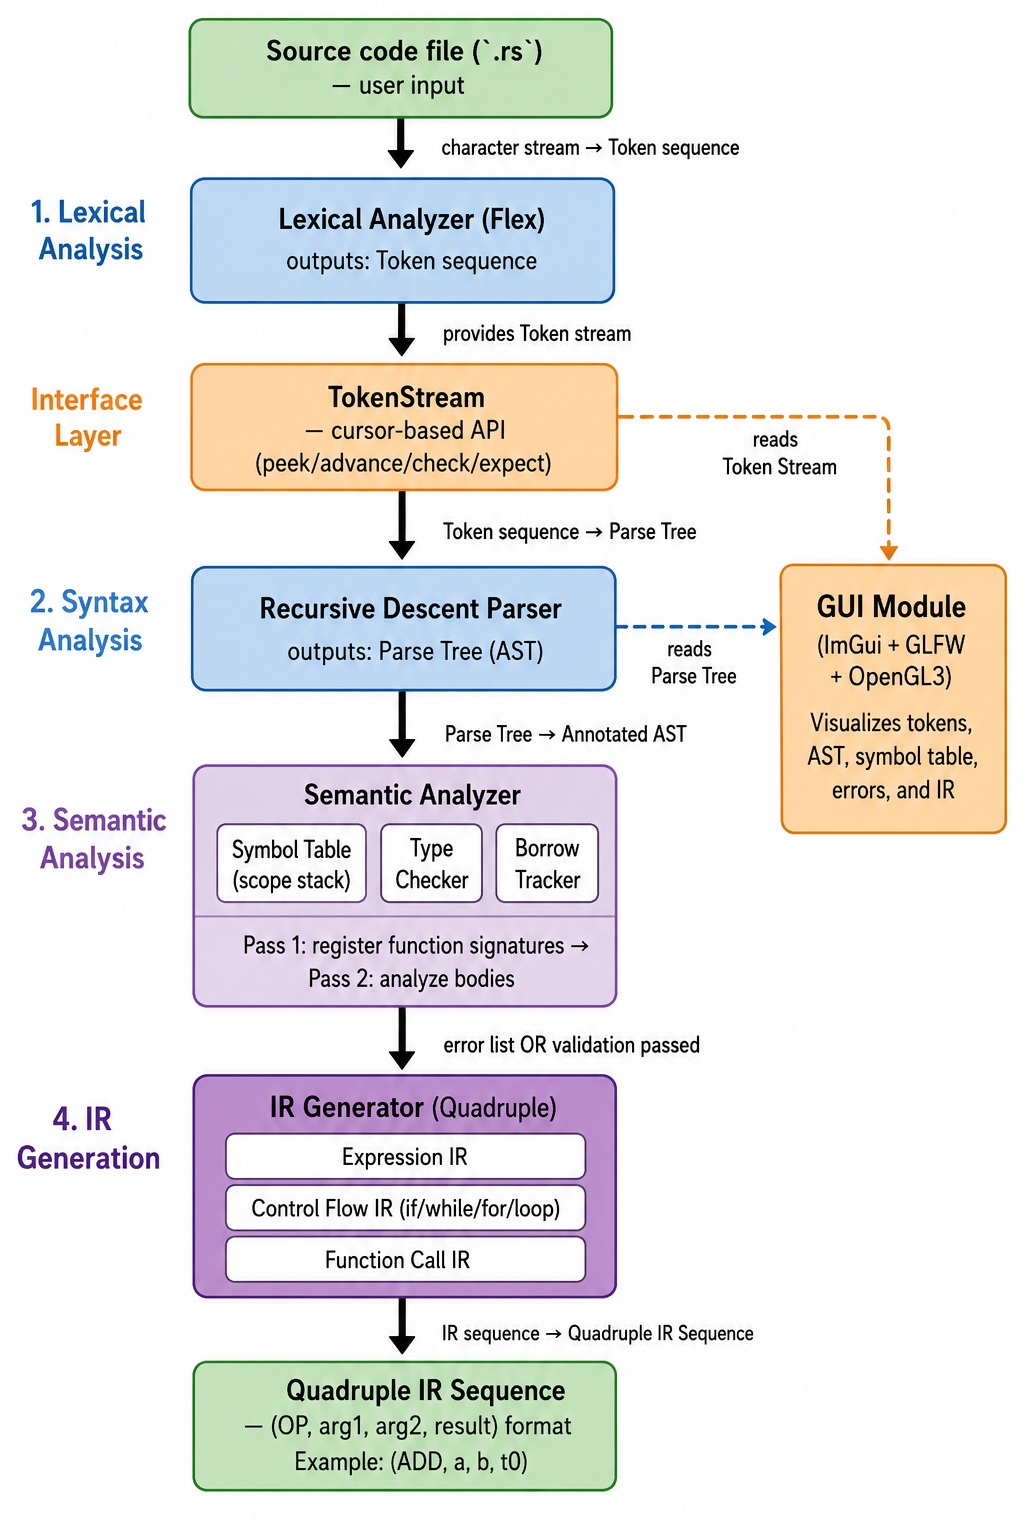
\includegraphics[width=\textwidth]{screenshot001}
\caption{系统总体架构图（含语义分析与中间代码生成）}
\label{fig:system_architecture_v2}
\end{figure}

\subsubsection{语义分析器 (SemanticAnalyzer)}

语义分析器继承了大作业1中讨论的"语义约束"检测思路，实现了完整的类型检查和语义错误诊断。主要功能包括：
\begin{itemize}
    \item \textbf{符号表管理}：使用栈式作用域，支持变量声明、查询、shadowing
    \item \textbf{类型系统}：支持i32、bool、void、引用（\&T / \&mut T）、数组（[T;N]）、元组（(T1,T2,...)）共7种基础类型
    \item \textbf{类型检查}：表达式类型推导、赋值类型一致性、函数参数/返回值类型匹配
    \item \textbf{借用追踪}：不可变引用/可变引用的共存约束检查
    \item \textbf{错误诊断}：18类语义错误的检测与定位
\end{itemize}

\subsubsection{中间代码生成器 (IRGenerator)}

中间代码生成器在语义分析通过后运行，将语法树转换为四元式序列。主要设计决策包括：
\begin{itemize}
    \item \textbf{四元式形式}：(OP, arg1, arg2, result)，直观、易于理解和后续优化
    \item \textbf{临时变量管理}：自动生成t0, t1, t2...等临时变量持有中间计算结果
    \item \textbf{标签管理}：自动生成L0, L1, L2...等标签用于控制流跳转
    \item \textbf{27种操作码}：覆盖赋值、算术、比较、跳转、函数调用、数组索引、引用/解引用等
\end{itemize}

\subsection{团队分工与开发环境}

\begin{table}[H]
\centering
\caption{团队分工表}
\begin{tabular}{|c|c|l|}
\hline
\textbf{姓名} & \textbf{学号} & \textbf{主要分工} \\
\hline
程浩然 & 2351579 & 语义分析器设计实现（类型系统、符号表、18类错误检测）、\\
 & & 借用追踪机制、两遍扫描函数前向引用处理、测试用例编写 \\
\hline
黄艺鑫 & 2253797 & 中间代码生成器设计实现（四元式体系、控制流翻译）、\\
 & & 表达式IR生成（运算符优先级映射）、IR输出格式设计 \\
\hline
韦畅 & 2352628 & 实验报告撰写、语义规则整理与对照、测试用例设计验证、\\
 & & 文档与参考资料整理 \\
\hline
\end{tabular}
\end{table}

\begin{table}[H]
\centering
\caption{开发环境配置}
\begin{tabular}{|l|l|}
\hline
\textbf{组件} & \textbf{版本/说明} \\
\hline
操作系统 & Linux (Ubuntu 22.04) / Windows 11 \\
\hline
编译器 & GCC/G++ 11, C++17 \\
\hline
Flex版本 & 2.6.4 \\
\hline
CMake版本 & 3.22+ \\
\hline
容器环境 & Docker (Ubuntu 22.04 基础镜像) \\
\hline
GUI框架 & ImGui + GLFW + OpenGL3 (仅Windows) \\
\hline
\end{tabular}
\end{table}

\newpage

% ============================================================
%  第二章 语义分析器设计与实现
% ============================================================
\section{语义分析器设计与实现}

语义分析是编译过程的第三阶段，负责在语法树的基础上检查程序的静态语义正确性。本章详细介绍语义分析器的设计与实现。

\subsection{语义分析理论基础}

\subsubsection{语义分析的任务}

语义分析位于语法分析和中间代码生成之间，其核心任务是：
\begin{enumerate}
    \item \textbf{类型检查}：验证每个表达式、语句、声明的类型是否一致
    \item \textbf{作用域分析}：确定每个标识符的可见范围，处理变量声明与引用
    \item \textbf{控制流检查}：验证break/continue在循环内、return类型匹配等
    \item \textbf{借用规则检查}：验证Rust风格的所有权和借用规则
\end{enumerate}

\subsubsection{Visitor模式}

本项目的语义分析采用\textbf{Visitor模式}（访问者模式）实现。Visitor模式的核心思想是将操作（语义分析）与数据结构（语法树）分离：语法树节点提供accept方法接收Visitor，Visitor为每种节点类型提供对应的visit方法。

\begin{figure}[H]
\centering
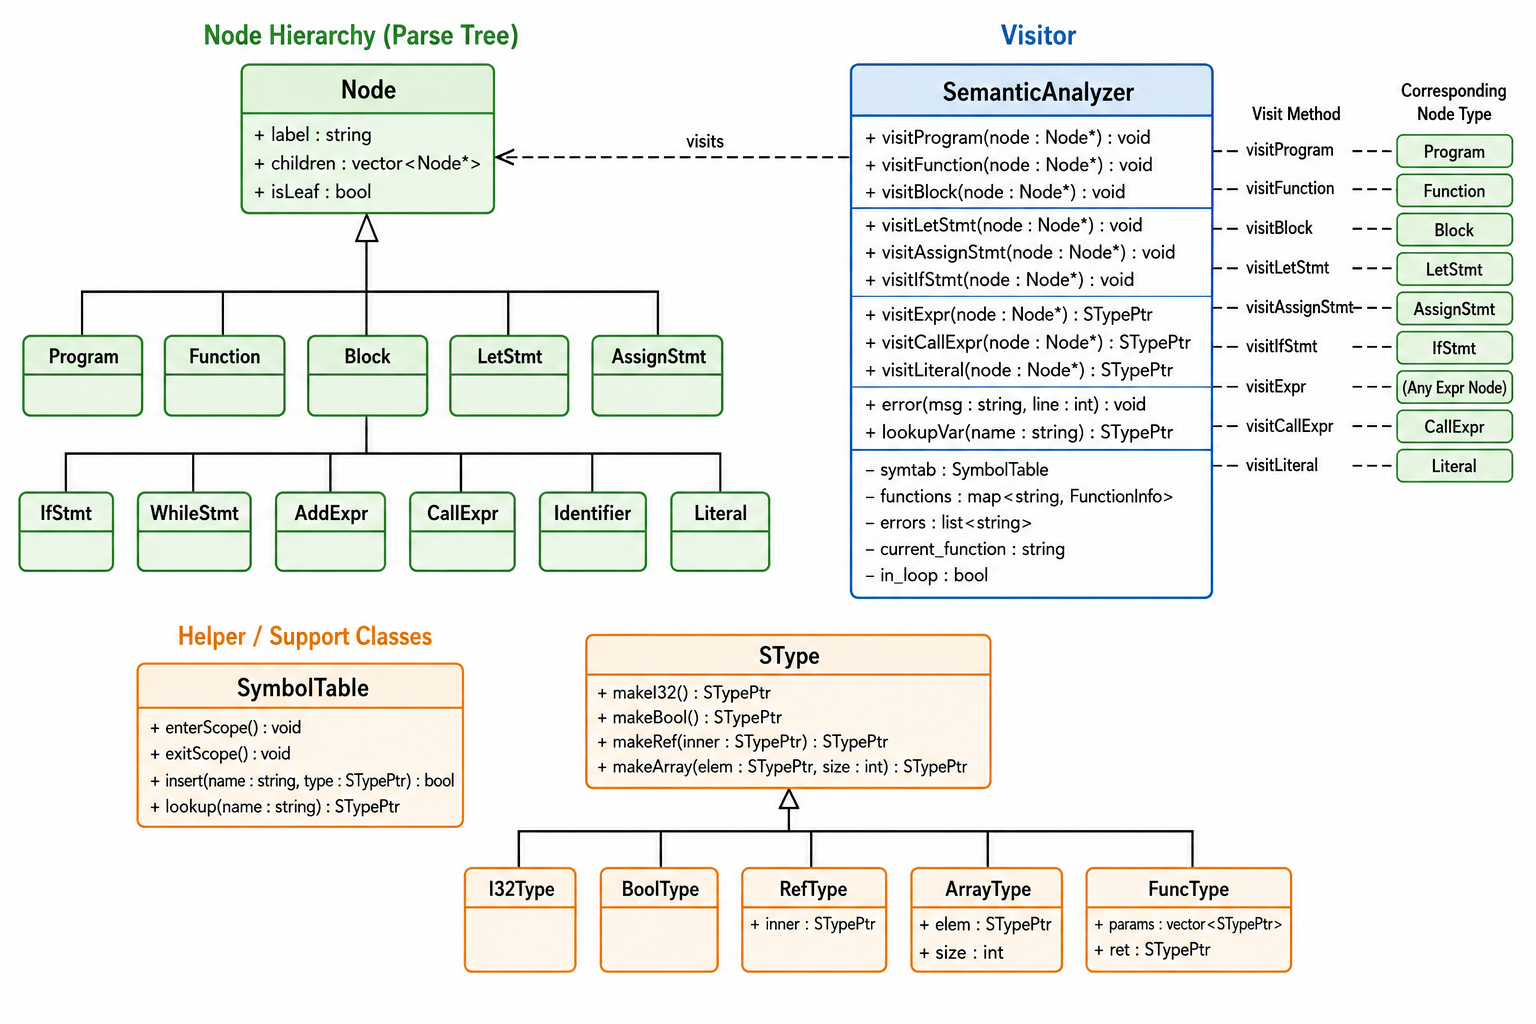
\includegraphics[width=0.8\linewidth]{screenshot002}
\caption{Visitor模式在语义分析中的应用}
\label{fig:visitor_pattern}
\end{figure}

在我们的实现中，Visitor模式体现为一系列visit函数：
\begin{lstlisting}[language=C++, caption={Visitor模式的函数声明}]
// 顶层访问
void visitProgram(const Node* node);
void visitFunction(const Node* node);
void visitBlock(const Node* node);
void visitStmt(const Node* node);

// 语句访问
void visitLetStmt(const Node* node);
void visitAssignStmt(const Node* node);
void visitReturnStmt(const Node* node);
void visitIfStmt(const Node* node);
// ...

// 表达式访问（返回类型信息）
STypePtr visitExpr(const Node* node);
STypePtr visitCmpExpr(const Node* node);
STypePtr visitCallExpr(const Node* node);
// ...
\end{lstlisting}

表达式Visitor返回类型信息（STypePtr），沿语法树自底向上传播，实现类型推导和类型检查。

\textbf{Visitor模式的工作机制}可以通过一个具体例子来理解。考虑语句 \texttt{let mut x = a + 1;} 的语义分析过程：

\begin{enumerate}
    \item \texttt{visitStmt()} 遇到 LetStmt 节点 → 分发到 \texttt{visitLetStmt()}
    \item \texttt{visitLetStmt()} 提取变量名 "x"，检测到无类型注解（类型初始为 UNKNOWN），检测到有初始化表达式
    \item 对初始化表达式子树调用 \texttt{visitExpr()}：
        \begin{itemize}
            \item 遇到 AddExpr 节点 → 分发到 \texttt{visitAddExpr()}
            \item \texttt{visitAddExpr()} 对左操作数调用 \texttt{visitExpr()}：
                \begin{itemize}
                    \item 遇到 Identifier("a") → \texttt{lookupVar("a")} → 返回 Symbol(类型=ST\_I32, is\_assigned=true)
                    \item \texttt{visitAtom()} 返回 ST\_I32
                \end{itemize}
            \item 对右操作数调用 \texttt{visitExpr()}：
                \begin{itemize}
                    \item 遇到 Literal(1) → \texttt{visitLiteral()} → 返回 ST\_I32
                \end{itemize}
            \item 检查左操作数类型(ST\_I32)与右操作数类型(ST\_I32)是否一致 → 一致
            \item \texttt{visitAddExpr()} 返回 ST\_I32（算术运算的结果类型）
        \end{itemize}
    \item \texttt{visitLetStmt()} 收到 initType = ST\_I32
    \item 变量 x 的类型从 UNKNOWN 更新为 ST\_I32（类型推导完成）
    \item 创建 Symbol("x", ST\_I32, mut=true, is\_assigned=true) 并插入符号表
\end{enumerate}

这个例子展示了Visitor模式的核心优势：\textbf{类型信息沿着语法树结构自底向上自然流动}，每个visit函数只需关注自己这一层的处理逻辑，下层细节被递归调用封装。

\subsection{类型系统设计}

\subsubsection{类型体系}

类型系统是语义分析的核心。我们设计了完整的基础类型层次结构：

\begin{figure}[H]
\centering
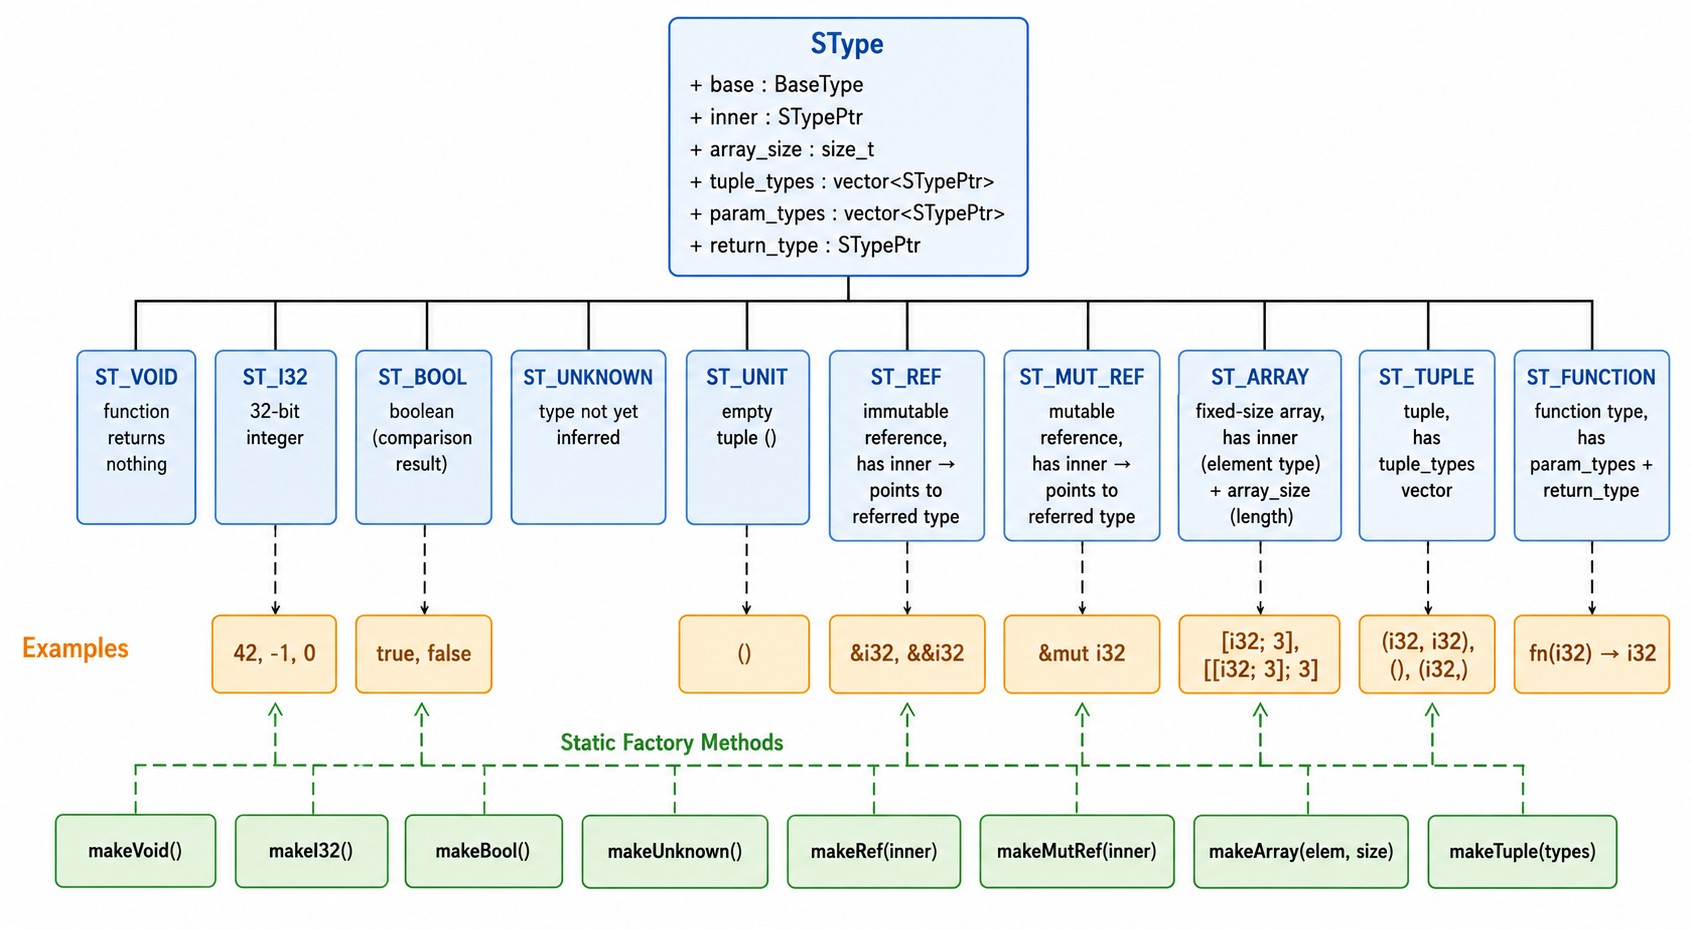
\includegraphics[width=\textwidth]{screenshot004}
\caption{语义类型系统层次结构}
\label{fig:type_hierarchy}
\end{figure}


\begin{table}[H]
\centering
\caption{基础类型（BaseType）枚举}
\begin{tabular}{|l|l|l|}
\hline
\textbf{BaseType} & \textbf{说明} & \textbf{示例} \\
\hline
ST\_VOID & 空类型（无返回值） & 函数返回void \\
\hline
ST\_I32 & 32位整数 & i32 \\
\hline
ST\_BOOL & 布尔类型（比较运算结果） & 1==1 的类型 \\
\hline
ST\_REF & 不可变引用 & \&i32 \\
\hline
ST\_MUT\_REF & 可变引用 & \&mut i32 \\
\hline
ST\_ARRAY & 定长数组 & [i32; 3] \\
\hline
ST\_TUPLE & 元组 & (i32, i32) \\
\hline
ST\_UNIT & 单元类型（空元组） & () \\
\hline
ST\_FUNCTION & 函数类型 & fn(i32) -> i32 \\
\hline
ST\_UNKNOWN & 未知类型（类型推导暂未完成） & 声明时未指定类型 \\
\hline
\end{tabular}
\end{table}

\subsubsection{类型定义与工厂方法}

\begin{lstlisting}[language=C++, caption={SType类定义}]
class SType {
public:
    BaseType base = BaseType::ST_UNKNOWN;  // 基础类型
    STypePtr inner;                         // 引用/数组的内部类型
    int array_size = 0;                     // 数组大小
    vector<STypePtr> tuple_types;           // 元组元素类型
    vector<STypePtr> param_types;           // 函数参数类型
    STypePtr return_type;                   // 函数返回类型

    // 工厂方法
    static STypePtr makeVoid();
    static STypePtr makeI32();
    static STypePtr makeBool();
    static STypePtr makeRef(STypePtr inner);
    static STypePtr makeMutRef(STypePtr inner);
    static STypePtr makeArray(STypePtr elem, int size);
    static STypePtr makeTuple(vector<STypePtr> types);
    static STypePtr makeUnknown();

    // 类型判断
    bool isI32() const;
    bool isBool() const;
    bool isRef() const;
    bool isArray() const;
    // ...

    // 类型比较
    bool equals(const STypePtr& other) const;
    string toString() const;
};
\end{lstlisting}

工厂方法模式使类型创建语义清晰，避免手动设置内部状态可能导致的错误。

\subsubsection{类型从语法树节点的解析}

类型信息出现在源代码的多个位置：变量声明、函数参数、返回类型等。所有这些位置都通过 \texttt{parseTypeFromNode()} 方法统一处理：

\begin{lstlisting}[language=C++, caption={类型解析逻辑}]
STypePtr parseTypeFromNode(const Node* node) {
    // 需要 Type 标签
    if (!node || node->label != "Type") return SType::makeUnknown();

    auto& first = node->children[0];

    // i32 -> ST_I32
    if (isLeafCat(first, "I32")) return SType::makeI32();

    // &T -> ST_REF, &mut T -> ST_MUT_REF
    if (isLeafCat(first, "Ampersand")) { /* ... */ }

    // [T; N] -> ST_ARRAY
    if (isLeafCat(first, "LBracket")) { /* ... */ }

    // (T1, T2, ...) -> ST_TUPLE
    if (isLeafCat(first, "LParen")) { /* ... */ }

    return SType::makeUnknown();
}
\end{lstlisting}

该方法递归解析嵌套类型，例如 \texttt{[[i32;3];3]} 会被解析为 ST\_ARRAY(inner=ST\_ARRAY(inner=ST\_I32, size=3), size=3)。

\subsubsection{类型等价性判断}

类型检查的核心操作是判断两个类型是否兼容。我们实现了\texttt{equals()}方法来进行结构化的类型比较：

\begin{lstlisting}[language=C++, caption={类型等价性判断}]
bool SType::equals(const STypePtr& other) const {
    if (!other) return false;
    if (base != other->base) return false;

    switch (base) {
    case BaseType::ST_REF:
    case BaseType::ST_MUT_REF:
        // 引用类型：要求内部类型相同，且引用类别相同
        return inner && other->inner && inner->equals(other->inner);

    case BaseType::ST_ARRAY:
        // 数组类型：要求元素类型相同 且 长度相同
        return array_size == other->array_size
            && inner && other->inner && inner->equals(other->inner);

    case BaseType::ST_TUPLE:
        // 元组类型：要求每个位置的元素类型一一对应相同
        if (tuple_types.size() != other->tuple_types.size())
            return false;
        for (size_t i = 0; i < tuple_types.size(); i++)
            if (!tuple_types[i]->equals(other->tuple_types[i]))
                return false;
        return true;

    default:
        // 基础类型（VOID/I32/BOOL/UNIT/UNKNOWN）：直接比较枚举值
        return true;
    }
}
\end{lstlisting}

类型等价判断的设计要点：
\begin{itemize}
    \item \textbf{结构等价}（Structural Equivalence）：不是比较类型名称（名字等价），而是递归比较类型的内部结构。例如两个\texttt{[i32; 3]}即使来源于不同的类型声明，也被判定为同一类型
    \item \textbf{引用类别敏感}：不可变引用\texttt{\&T}和可变引用\texttt{\&mut T}是不等价的，即使内部类型T相同
    \item \textbf{ST\_UNKNOWN宽松匹配}：当某一侧的类型尚为UNKNOWN（如未初始化的类型推导），\texttt{equals()}在该侧成立时返回true，避免在类型推导完成前误报错误
\end{itemize}

\subsubsection{类型推导机制}

当变量声明未指定类型时（如\texttt{let mut b;}），语义分析器需要通过后续的赋值来推导类型。我们采用以下策略：

\begin{enumerate}
    \item \textbf{声明时标记为UNKNOWN}：变量初次声明时类型设为ST\_UNKNOWN
    \item \textbf{首次赋值触发推导}：当对UNKNOWN类型变量赋值时，变量类型更新为赋值表达式的类型
    \item \textbf{后续赋值做类型检查}：类型确定后，后续赋值需进行常规的类型一致性检查
    \item \textbf{使用前检查}：如果变量在类型推导完成前就被作为右值使用（\texttt{is\_assigned == false}），报告"变量使用前未赋值"错误
\end{enumerate}

这种设计模拟了Rust编译器的类型推导行为：局部变量的类型可以根据首次使用的上下文自动推导，不需要显式标注。

\subsection{符号表设计}

\subsubsection{符号表条目}

每个声明的变量在符号表中对应一个Symbol条目：

\begin{lstlisting}[language=C++, caption={Symbol结构体}]
struct Symbol {
    string name;                // 变量名
    STypePtr type;              // 变量类型
    bool is_mutable;            // 是否可变 (mut)
    bool is_assigned;           // 是否已被赋值
    int scope_level;            // 声明所在作用域层级
    int line;                   // 声明行号
    bool has_immutable_ref;     // 是否存在不可变引用 (借用追踪)
    bool has_mutable_ref;       // 是否存在可变引用 (借用追踪)
};
\end{lstlisting}

\subsubsection{栈式作用域}

符号表采用\textbf{栈式作用域}（Stack of HashMaps）实现：

\begin{figure}[H]
\centering
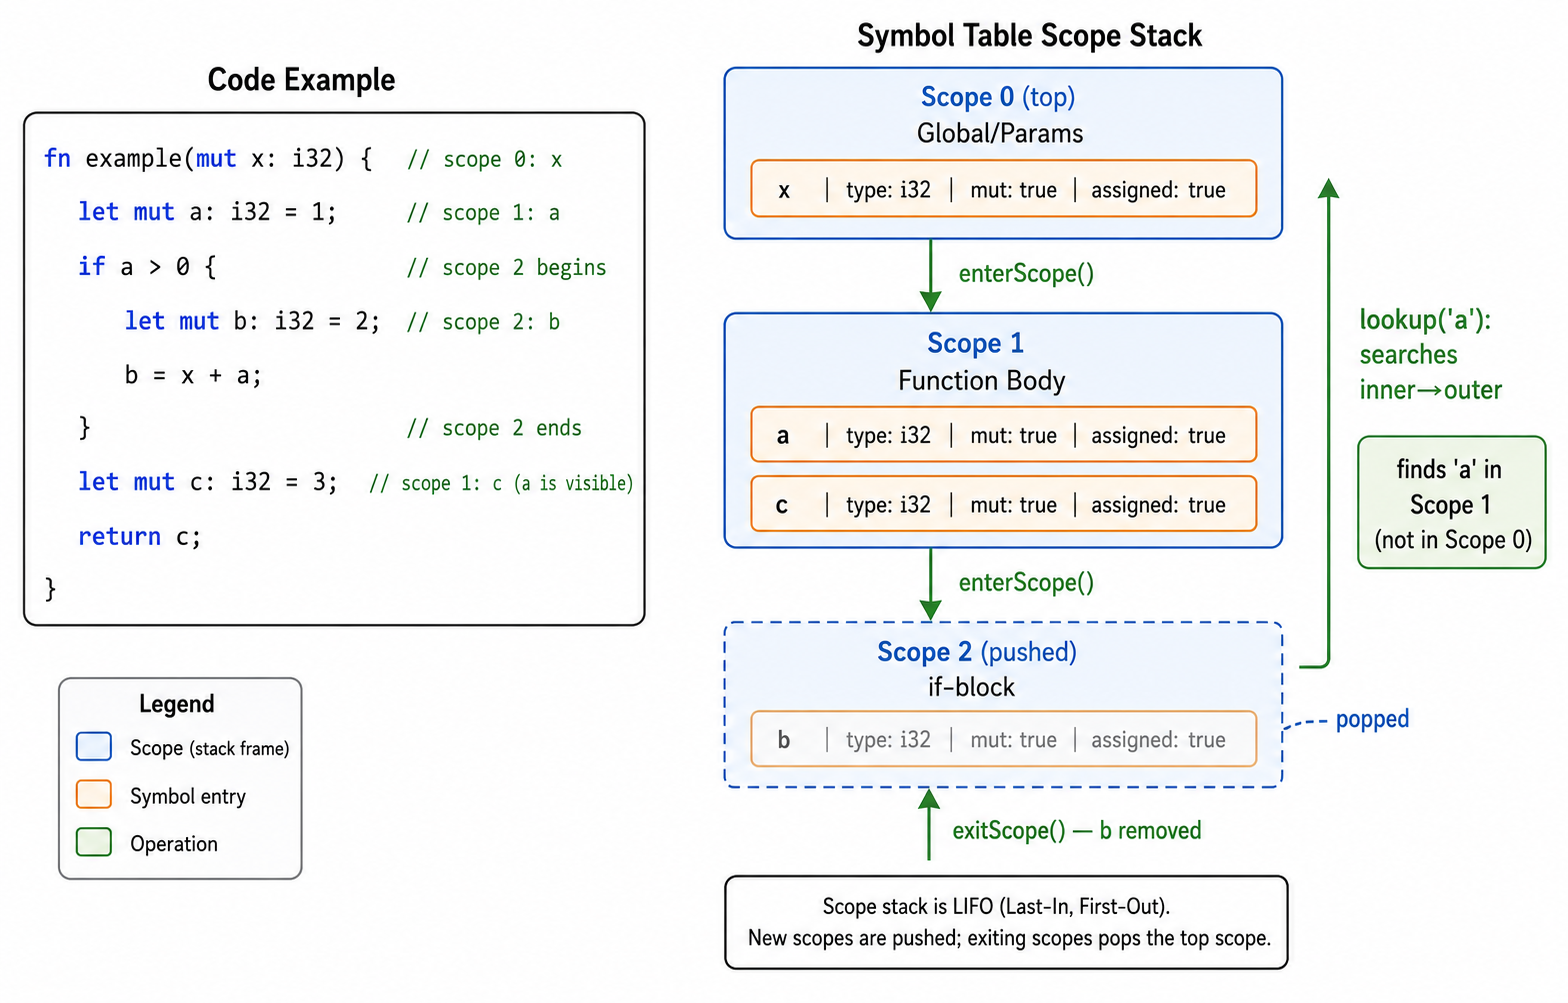
\includegraphics[width=0.75\linewidth]{screenshot005}
\caption{符号表栈式作用域结构}
\label{fig:symbol_table}
\end{figure}


\begin{lstlisting}[language=C++, caption={SymbolTable实现}]
class SymbolTable {
    vector<unordered_map<string, shared_ptr<Symbol>>> scopes;
    int current_scope = 0;

    void enterScope() {
        current_scope++;
        scopes.emplace_back();  // 压入新作用域
    }

    void exitScope() {
        scopes.pop_back();      // 弹出当前作用域
        current_scope--;
    }

    shared_ptr<Symbol> lookup(const string& name) const {
        // 从内向外逐层查找
        for (int i = scopes.size() - 1; i >= 0; i--) {
            auto it = scopes[i].find(name);
            if (it != scopes[i].end()) return it->second;
        }
        return nullptr;  // 未找到
    }
};
\end{lstlisting}

栈式作用域的设计特点：
\begin{itemize}
    \item \textbf{作用域嵌套}：每个 \texttt{\{...\}} 块创建新的作用域层
    \item \textbf{从内向外查找}：\texttt{lookup()} 从最内层开始向外搜索，自然实现变量遮蔽
    \item \textbf{Shadowing支持}：\texttt{insert()} 直接覆盖当前作用域中的同名变量，实现Rust风格的重影（shadowing）
    \item \textbf{退出即清理}：离开作用域时弹出栈顶，自动释放该作用域内的所有变量
\end{itemize}

\subsubsection{函数信息管理}

函数信息使用独立的HashMap管理（不随作用域消除），存储函数签名供调用点检查：

\begin{lstlisting}[language=C++, caption={FunctionInfo结构体}]
struct FunctionInfo {
    string name;                              // 函数名
    vector<pair<string, STypePtr>> params;    // 形参列表 (name, type)
    STypePtr return_type;                     // 返回类型
    int line;                                 // 声明行号
};
\end{lstlisting}

\subsection{两遍扫描处理函数前向引用}

本项目的一个重要设计是\textbf{两遍扫描}（Two-Pass）策略，允许函数在定义之前被调用：

\begin{figure}[H]
\centering
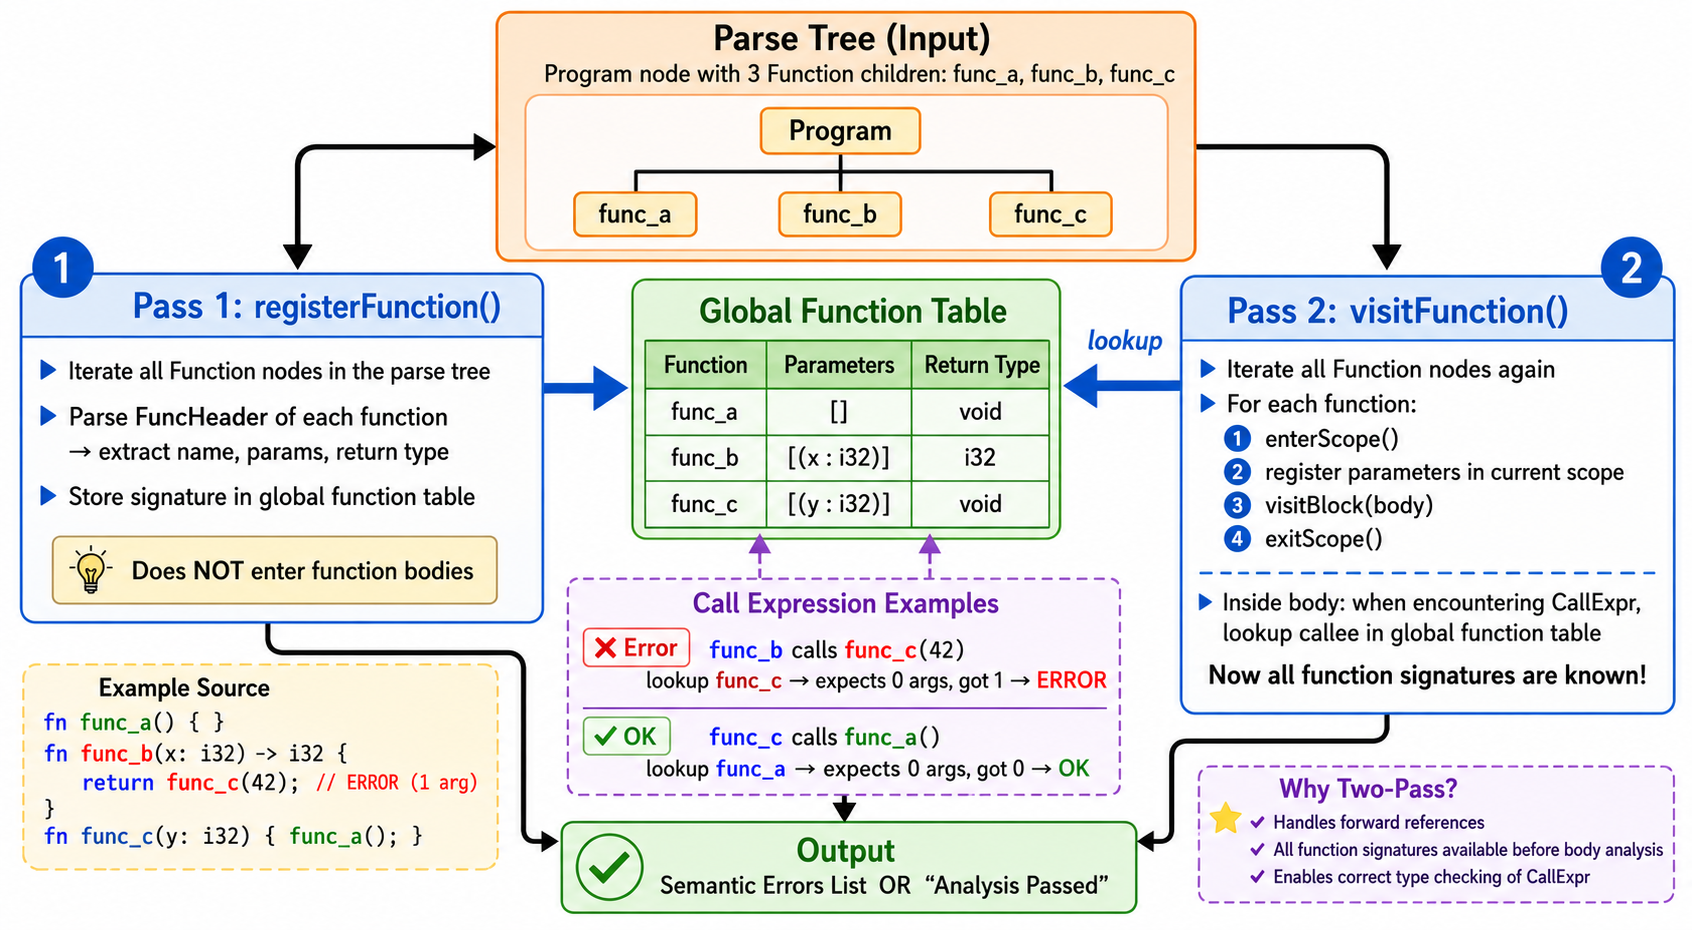
\includegraphics[width=\textwidth]{screenshot006}
\caption{两遍扫描策略处理函数前向引用}
\label{fig:two_pass_scan}
\end{figure}


\begin{lstlisting}[language=C++, caption={两遍扫描实现}]
void visitProgram(const Node* node) {
    auto funcNodes = findChildren(node, "Function");

    // Pass 1: 注册所有函数签名（不分析函数体）
    for (auto* fn : funcNodes)
        registerFunction(fn);

    // Pass 2: 分析所有函数体（此时所有函数签名已知）
    for (auto* fn : funcNodes)
        visitFunction(fn);
}
\end{lstlisting}

\textbf{第一遍}调用 \texttt{registerFunction()}，解析每个函数的头声明（函数名、形参类型、返回类型），将签名存入全局函数表。此时不进入函数体，不分析任何表达式。

\textbf{第二遍}调用 \texttt{visitFunction()}，此时所有函数签名都已注册，函数体中的任何调用都能在全局表中找到目标函数的签名，从而正确检查参数数量和类型。

这种设计消除了C语言中需要"前向声明"的限制，使编译器更接近现代语言的行为。

\subsection{语义错误检测}

\subsubsection{错误检测总览}

本项目的语义分析器能够检测\textbf{18类语义错误}，覆盖作业要求的所有场景：

\begin{table}[!htp]
\centering
\caption{语义错误检测列表}
\label{tab:semantic_errors}
\begin{tabular}{|c|l|l|l|}
\hline
\textbf{编号} & \textbf{错误类型} & \textbf{对应规则} & \textbf{示例} \\
\hline
1 & 返回类型不一致 (void→i32) & 1.5 & \texttt{fn f()->i32 \{ return;\}} \\
\hline
2 & 返回类型不一致 (i32→void) & 1.5 & \texttt{fn f() \{ return 1;\}} \\
\hline
3 & 赋值给未声明变量 & 2.2 & \texttt{a=32;}（a未声明） \\
\hline
4 & 赋值类型不一致 & 2.2 & \texttt{let mut a:i32; a=1==1;} \\
\hline
5 & 右值未提前声明 & 2.2 & \texttt{let mut b:i32=a;}（a未声明） \\
\hline
6 & 右值未提前赋值 & 2.2 & \texttt{let mut a:i32; let b:i32=a;} \\
\hline
7 & 不可变变量二次赋值 & 6.1 & \texttt{let c:i32=1; c=2;} \\
\hline
8 & 实参数量不一致 & 3.5 & \texttt{f(1)}（f无参数） \\
\hline
9 & 无返回值函数作为右值 & 3.5 & \texttt{let mut a=void\_func();} \\
\hline
10 & 实参类型不一致 & 3.5 & \texttt{f(1==1)}（f期望i32） \\
\hline
11 & break不在循环体内 & 5.4 & 函数中直接\texttt{break;} \\
\hline
12 & continue不在循环体内 & 5.4 & 函数中直接\texttt{continue;} \\
\hline
13 & 可变引用与其他引用共存 & 6.3 & \texttt{\&a}和\texttt{\&mut a}同时存在 \\
\hline
14 & 从不可变变量创建可变引用 & 6.3 & \texttt{let a:i32=1; let mut b=\&mut a;} \\
\hline
15 & 对非引用类型解引用 & 6.4 & \texttt{let mut b=*a;}（a非ref） \\
\hline
16 & 不可变引用修改指向数据 & 6.4 & \texttt{let b=\&a; *b=2;} \\
\hline
17 & 数组初始化元素数量不一致 & 8.2 & \texttt{a=[1,2,3];}（a声明为[i32;2]） \\
\hline
18 & 元组初始化元素数量不一致 & 9.2 & \texttt{a=(1,2,3);}（a声明为(i32,i32)） \\
\hline
\end{tabular}
\end{table}

\subsubsection{类型检查实现}

类型检查的核心是\textbf{类型一致性判断}。在赋值、参数传递、返回语句等位置，比较期望类型与实际类型。下面以赋值语句为例展示完整的类型检查流程：

\begin{lstlisting}[language=C++, caption={赋值语句的完整类型检查实现}]
void visitAssignStmt(const Node* node) {
    int line = extractLine(node);
    // 步骤1: 找到赋值号的位置
    int assignIdx = -1;
    for (size_t i = 0; i < node->children.size(); i++) {
        if (isLeafCat(node->children[i].get(), "Assign")) {
            assignIdx = (int)i; break;
        }
    }
    if (assignIdx < 0) return;

    auto* lhsNode = node->children[0].get();

    // 步骤2: 检查左值声明状态
    // 对于标识符左值: a = expr  或  *p = expr
    // 对于数组下标: arr[0] = expr
    checkLvalue(lhsNode, line);

    // 步骤3: 左值类型推导 + 可变性检查
    STypePtr lhsType;
    if (lhsNode->label == "Identifier") {
        string name = extractId(lhsNode);
        auto sym = symtab.lookup(name);
        if (sym) {
            lhsType = sym->type;
            // 检查可变性
            if (!sym->is_mutable)
                error("cannot assign to immutable variable", line);
            // 检查不可变引用赋值
            if (sym->type->isRef() && !sym->type->isMutRef())
                error("cannot assign through immutable reference", line);
        }
    } else {
        lhsType = visitExpr(lhsNode); // DerefExpr / IndexExpr
    }

    // 步骤4: 右值类型推导
    auto rhsType = visitExpr(node->children[assignIdx + 1].get());

    // 步骤5: 类型一致性检查
    if (lhsType && !lhsType->isUnknown()
        && !rhsType->isUnknown()
        && !lhsType->equals(rhsType)) {
        error("type mismatch in assignment: " +
              lhsType->toString() + " vs " + rhsType->toString(), line);
    }

    // 步骤6: 标记变量为已赋值
    if (lhsNode->label == "Identifier") {
        string name = extractId(lhsNode);
        auto sym = symtab.lookup(name);
        if (sym) sym->is_assigned = true;
    }
}
\end{lstlisting}

\textbf{类型传播机制}：表达式类型沿语法树自底向上传播——字面量返回对应的类型（整数常量→ST\_I32），标识符从符号表查找类型（未声明→报错，未赋值→报错），比较运算始终返回ST\_BOOL，算术运算要求操作数类型一致并返回操作数类型，函数调用返回函数声明的返回类型。

下面以三个典型场景为例，展示类型检查的完整数据流：

\textbf{场景一：基本赋值} \texttt{a = 42}（a为\texttt{let mut a:i32}）
\begin{enumerate}
    \item checkLvalue("a") → 查符号表，a存在且声明为mut → 通过
    \item 求lhsType → lookup("a") → ST\_I32
    \item 求rhsType → visitExpr(42) → visitLiteral → ST\_I32
    \item equals(ST\_I32, ST\_I32) → true → 通过类型检查
    \item 标记a.is\_assigned = true
\end{enumerate}

\textbf{场景二：类型不匹配} \texttt{a = 1==1}（a为\texttt{let mut a:i32}）
\begin{enumerate}
    \item checkLvalue("a") → 通过
    \item lhsType = ST\_I32
    \item visitExpr(1==1) → visitCmpExpr → 左右操作数均为ST\_I32 → 返回ST\_BOOL
    \item rhType = ST\_BOOL
    \item equals(ST\_I32, ST\_BOOL) → false → 报错"type mismatch: i32 vs bool"
\end{enumerate}

\textbf{场景三：类型推导} \texttt{let mut b; b = 42}
\begin{enumerate}
    \item visitLetStmt → b的类型初始为ST\_UNKNOWN（未指定类型注解）
    \item visitAssignStmt → lhsType = ST\_UNKNOWN
    \item rhsType = ST\_I32
    \item equals条件：lhsType是UNKNOWN → 跳过类型检查（不报错）
    \item 同时b.is\_assigned更新为true，b.type从ST\_UNKNOWN更新为ST\_I32
\end{enumerate}

\subsubsection{借用追踪实现}

借用追踪模拟了Rust的所有权规则，通过符号表中的\texttt{has\_immutable\_ref}和\texttt{has\_mutable\_ref}标志位实现：

\begin{lstlisting}[language=C++, caption={借用追踪逻辑}]
STypePtr visitRefExpr(const Node* node) {
    // ...
    if (is_mut) {
        // 创建 &mut：检查是否有其他引用存在
        if (sym->has_immutable_ref || sym->has_mutable_ref)
            error("cannot create mutable reference: other refs exist");
        sym->has_mutable_ref = true;
    } else {
        // 创建 &：检查是否有可变引用存在
        if (sym->has_mutable_ref)
            error("cannot create immutable ref: mutable ref exists");
        sym->has_immutable_ref = true;
    }
    // ...
}
\end{lstlisting}

借用规则总结：
\begin{itemize}
    \item \textbf{多个不可变引用}允许多个 \texttt{\&T} 同时存在
    \item \textbf{可变引用独占}存在 \texttt{\&mut T} 时，不能有任何其他引用
    \item \textbf{只能从可变变量创建可变引用}let a 不能创建 \texttt{\&mut a}
    \item \textbf{不可变引用不能修改数据}\texttt{*b=2} 在 b 为 \texttt{\&T} 时报错
\end{itemize}

\subsubsection{循环深度计数与控制流检查}

break和continue必须出现在循环体内，这一检查通过一个简单的计数器实现：

\begin{lstlisting}[language=C++, caption={in\_loop计数器管理}]
int in_loop = 0;  // 当前所在的循环嵌套深度

// 进入循环时递增
void visitWhileStmt(const Node* node) {
    // ... 检查条件表达式 ...
    in_loop++;
    visitBlock(bodyBlock);
    in_loop--;
}

// break/continue时检查
void visitBreakStmt(const Node* node) {
    if (in_loop <= 0)
        error("break statement must be inside a loop", line);
}
void visitContinueStmt(const Node* node) {
    if (in_loop <= 0)
        error("continue statement must be inside a loop", line);
}
\end{lstlisting}

\texttt{in\_loop}本质上是一个语义分析专用的``上下文标志''，与IR生成阶段的break\_label/continue\_label形成了清晰的职责分离：语义分析负责检查``是否在循环内''的合法性，IR生成负责实现``跳转到正确目标''的语义。

\subsubsection{复合类型的匹配检查}

数组和元组类型的语义检查涉及两个维度：\textbf{类型维度}（元素类型是否匹配）和\textbf{数量维度}（元素个数是否一致）。

\textbf{数组初始化检查}—以\texttt{let mut a:[i32;2]; a=[1,2,3];}为例：
\begin{itemize}
    \item 左值类型：通过parseTypeFromNode解析得到ST\_ARRAY(inner=ST\_I32, size=2)
    \item 右值类型：visitArrayLit遍历三个元素，每个返回ST\_I32，构造类型为ST\_ARRAY(inner=ST\_I32, size=3)
    \item equals(ST\_ARRAY(i32,2), ST\_ARRAY(i32,3)) → array\_size 2≠3 → false → 报错
\end{itemize}

\textbf{元组初始化检查}—以\texttt{let mut a:(i32,i32); a=(1,2,3);}为例：
\begin{itemize}
    \item 左值类型：ST\_TUPLE with types [ST\_I32, ST\_I32]
    \item 右值类型：visitTupleLit遍历三个元素后，构造ST\_TUPLE with types [ST\_I32, ST\_I32, ST\_I32]
    \item equals比较时，先比较tuple\_types.size()（2≠3），立即返回false → 报错
\end{itemize}

这种结构化比较自然地处理了嵌套复合类型，例如\texttt{[[i32;2];3]}与\texttt{[[i32;3];2]}虽然总元素数相同（6个），但由于数组长度不同（2≠3），类型比较会返回false。

\subsubsection{左值检查详解}

左值（Lvalue）是可以出现在赋值号左侧的表达式。我们的语言中，合法的左值包括：
\begin{itemize}
    \item \textbf{标识符}：\texttt{a}（前提：已声明且可变）
    \item \textbf{数组下标}：\texttt{arr[0]}（前提：数组变量可变）
    \item \textbf{解引用}：\texttt{*ptr}（前提：ptr为可变引用）
    \item \textbf{元组字段}：\texttt{tup.0}（前提：元组变量可变）
\end{itemize}

\texttt{checkLvalue()}方法递归检查左值的有效性：

\begin{lstlisting}[language=C++, caption={左值检查实现}]
void SemanticAnalyzer::checkLvalue(const Node* node, int line) {
    if (node->label == "Identifier") {
        // 简单变量: 检查是否已声明
        string name = extractId(node);
        auto sym = symtab.lookup(name);
        if (!sym) error("variable '" + name +
                        "' not declared", line);
        return;
    }

    if (node->label == "IndexExpr") {
        // 数组下标 arr[i]: 检查数组是否可变
        string name = extractId(node);
        auto sym = symtab.lookup(name);
        if (sym && !sym->is_mutable)
            error("cannot assign to element of "+
                  "immutable array", line);
        return;
    }

    if (node->label == "DerefExpr") {
        // 解引用 *ptr: 检查ptr是否为可变引用
        const Node* inner = nullptr;
        for (auto& c : node->children)
            if (!c->isLeaf) { inner = c.get(); break; }

        if (inner) {
            auto innerType = visitExpr(inner);
            if (innerType->isRef() && !innerType->isMutRef())
                error("cannot assign through "+
                      "immutable reference", line);
        }
        return;
    }
}
\end{lstlisting}

左值检查是语义分析的第一道防线——在检查类型匹配之前，先确保赋值的目标本身是合法的。

\subsection{语义分析流程总览}

\begin{figure}[!htp]
\centering
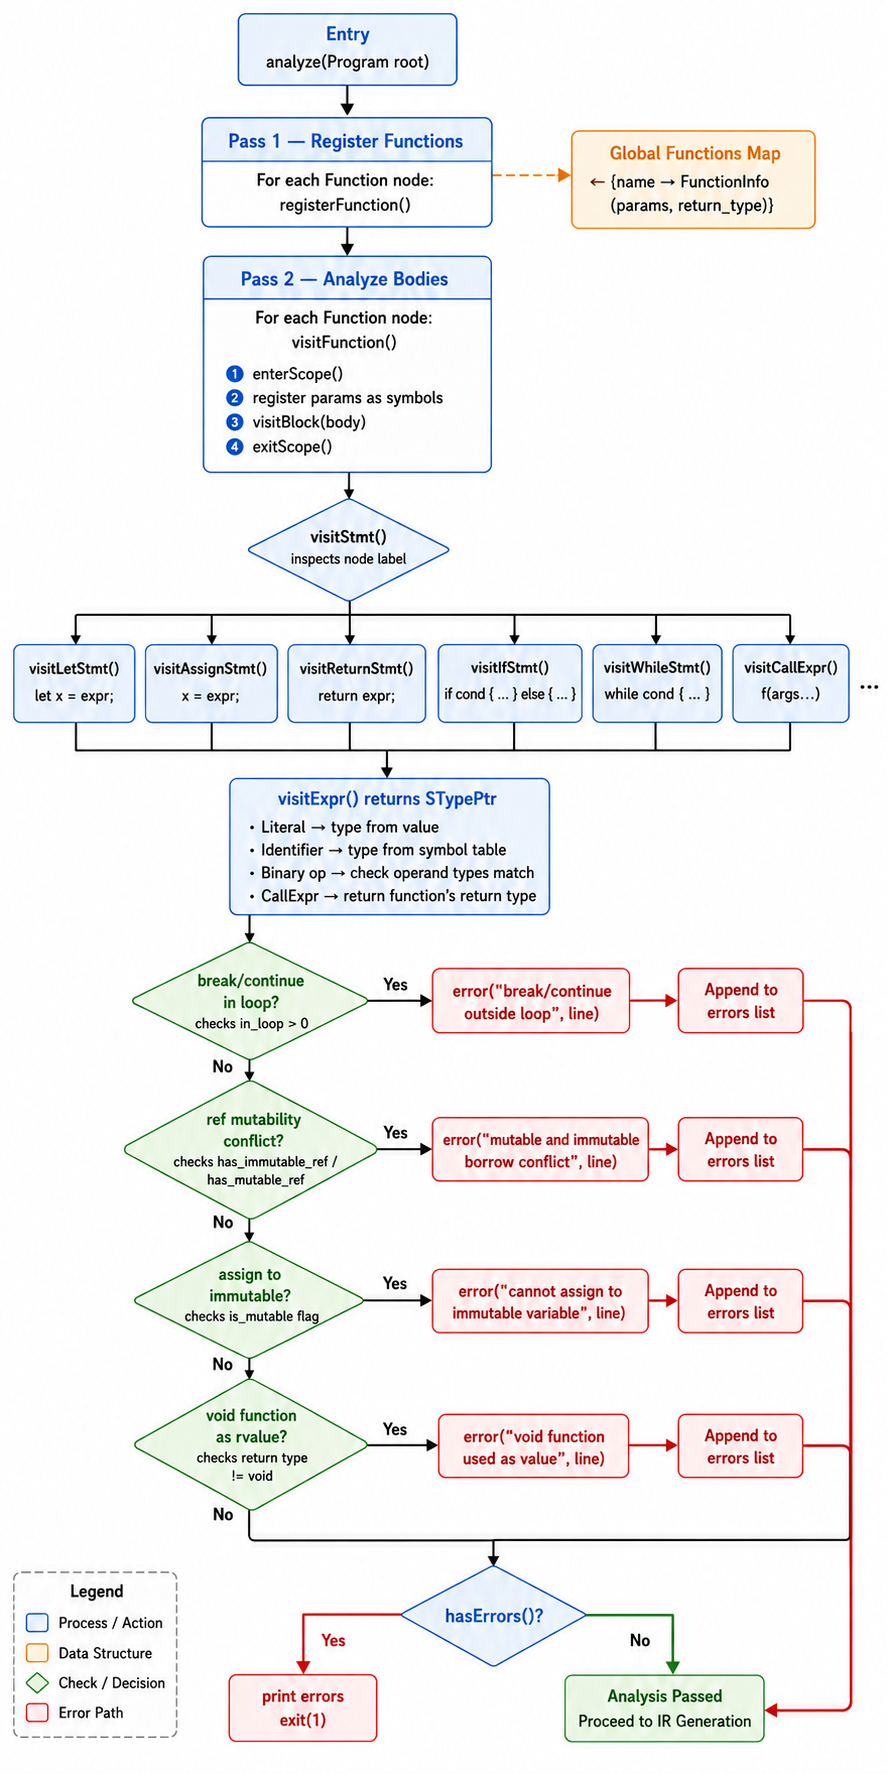
\includegraphics[width=0.7\textwidth]{screenshot007}
\caption{语义分析整体流程图}
\label{fig:semantic_flow}
\end{figure}


语义分析的完整流程：
\begin{enumerate}
    \item 语法树根节点 \texttt{Program} → \texttt{visitProgram()}
    \item 第一遍（Pass 1）：遍历所有Function节点，调用\texttt{registerFunction()}注册函数签名到全局函数表。此过程只解析函数头声明（函数名、形参类型、返回类型），不进入函数体
    \item 第二遍（Pass 2）：遍历所有Function节点，调用\texttt{visitFunction()}分析函数体。每个函数体内部：
        \begin{itemize}
            \item \texttt{enterScope()}：创建新的符号表作用域
            \item 注册形参：将每个参数作为Symbol插入符号表（预标记is\_assigned = true）
            \item \texttt{visitBlock(body)}：遍历语句序列
        \end{itemize}
    \item 每种语句：\texttt{visitStmt()}根据节点标签（LetStmt/AssignStmt/ReturnStmt/IfStmt/...）分发到对应的visit函数
    \item 每个表达式：对应的visit函数返回STypePtr，沿树向上传播类型信息。类型信息从叶子节点（字面量、标识符）向上汇聚到根节点
    \item 在关键位置（赋值的=号处、函数调用的实参处、return语句处）触发类型一致性检查
    \item 记录所有错误到内部的\texttt{vector<SemanticError>}列表，不中断分析
    \item 分析完成后统一输出所有错误；若存在任何错误，终止后续阶段
\end{enumerate}

\newpage

% ============================================================
%  第三章 中间代码生成器设计与实现
% ============================================================
\section{中间代码生成器设计与实现}

中间代码生成是编译过程的第四阶段，负责将经过语义检查的语法树转换为与目标机器无关的中间表示。本章详细介绍中间代码生成器的设计与实现。

\subsection{中间代码理论基础}

\subsubsection{为什么需要中间代码}

中间代码（Intermediate Representation, IR）是编译器前端和后端之间的桥梁：
\begin{itemize}
    \item \textbf{与源语言解耦}：不同高级语言可以生成相同的IR，共享后端
    \item \textbf{与目标机器解耦}：同一IR可以通过不同后端生成不同平台的机器码
    \item \textbf{便于优化}：IR形式简洁、语义明确，适合各种优化算法
    \item \textbf{便于理解和调试}：比汇编更接近源语言，比语法树更接近机器
\end{itemize}

\subsubsection{四元式（Quadruple）}

本项目选择\textbf{四元式}（Quadruple）作为中间代码的形式。四元式是三地址码的一种具体表示，每条指令包含四个字段：

$$(op,\ arg1,\ arg2,\ result)$$

其中：
\begin{itemize}
    \item \texttt{op}：操作码，指示要执行的操作
    \item \texttt{arg1}：第一操作数（变量名、临时变量、常量、标签）
    \item \texttt{arg2}：第二操作数（变量名、临时变量、常量、标签）
    \item \texttt{result}：结果存放位置（变量名或临时变量）
\end{itemize}

\begin{figure}[H]
\centering
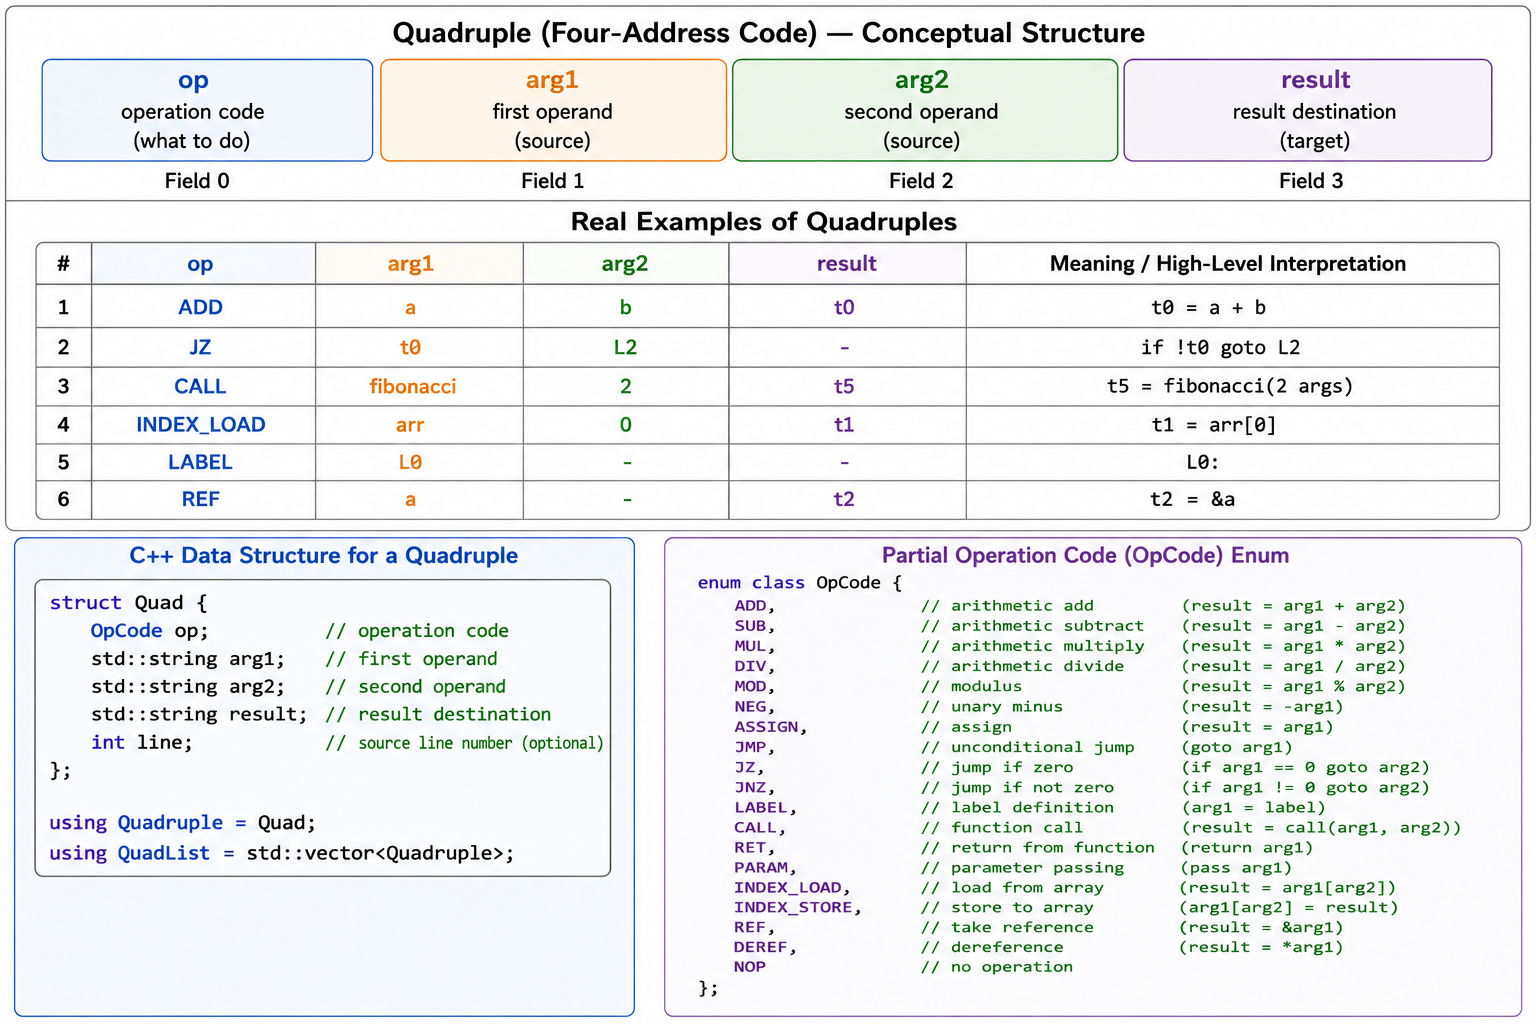
\includegraphics[width=0.8\linewidth]{screenshot008}
\caption{四元式结构示意图}
\label{fig:quadruple_structure}
\end{figure}


\subsection{IR操作码定义}

\begin{table}[H]
\centering
\caption{IR操作码（IROp）全集}
\begin{tabular}{|l|l|l|}
\hline
\textbf{分类} & \textbf{操作码} & \textbf{说明} \\
\hline
\multirow{5}{*}{算术运算} & ADD & 加法: result = arg1 + arg2 \\
& SUB & 减法: result = arg1 - arg2 \\
& MUL & 乘法: result = arg1 * arg2 \\
& DIV & 除法: result = arg1 / arg2 \\
& NEG & 取负: result = -arg1 \\
\hline
\multirow{6}{*}{比较运算} & EQ & 等于: result = (arg1 == arg2) \\
& NE & 不等: result = (arg1 != arg2) \\
& LT & 小于: result = (arg1 < arg2) \\
& LE & 小于等于: result = (arg1 <= arg2) \\
& GT & 大于: result = (arg1 > arg2) \\
& GE & 大于等于: result = (arg1 >= arg2) \\
\hline
\multirow{5}{*}{控制流} & LABEL & 标签定义（跳转目标） \\
& JUMP & 无条件跳转: goto arg1 \\
& JZ & 条件跳转: if !arg1 goto arg2 \\
& JNZ & 条件跳转: if arg1 goto arg2 \\
& NOP & 空操作 \\
\hline
\multirow{3}{*}{函数} & FUNC\_BEGIN & 函数开始 \\
& FUNC\_END & 函数结束 \\
& PARAM & 实参传递 \\
& CALL & 函数调用: result = arg1(arg2个参数) \\
& RETURN & 函数返回 \\
\hline
\multirow{6}{*}{数据操作} & ASSIGN & 赋值: result = arg1 \\
& INDEX\_LOAD & 数组读: result = arg1[arg2] \\
& INDEX\_STORE & 数组写: arg1[arg2] = result \\
& REF & 取引用: result = \&arg1 \\
& DEREF & 解引用: result = *arg1 \\
& TUPLE\_GET & 元组元素访问 \\
& ARRAY\_LIT & 数组字面量填充 \\
\hline
\multirow{2}{*}{循环控制} & BREAK & 跳出循环 \\
& CONTINUE & 继续下一次循环 \\
\hline
\end{tabular}
\end{table}

\subsection{四元式数据结构}

\begin{lstlisting}[language=C++, caption={四元式数据结构}]
enum class IROp {
    LABEL, ASSIGN, ADD, SUB, MUL, DIV,
    EQ, NE, LT, LE, GT, GE,
    JUMP, JZ, JNZ,
    PARAM, CALL, RETURN,
    INDEX_STORE, INDEX_LOAD,
    REF, DEREF,
    NEG, NOP,
    FUNC_BEGIN, FUNC_END,
    TUPLE_GET, ARRAY_LIT,
    BREAK, CONTINUE
};

struct Quadruple {
    IROp op;
    string arg1;    // 第一操作数（或标签名）
    string arg2;    // 第二操作数
    string result;  // 结果/目标

    string toString() const {
        // 格式: (OP, arg1, arg2, result)
        // 空值用 "-" 表示
    }
};
\end{lstlisting}

\subsection{IR生成器核心实现}

\subsubsection{临时变量与标签管理}

IR生成器内部维护两个计数器，自动生成唯一的临时变量名和标签名：

\begin{lstlisting}[language=C++, caption={临时变量与标签管理}]
class IRGenerator {
    int temp_counter = 0;   // 临时变量计数器
    int label_counter = 0;  // 标签计数器

    string newTemp() { return "t" + to_string(temp_counter++); }
    string newLabel() { return "L" + to_string(label_counter++); }

    void emit(IROp op, const string& a1="", const string& a2="",
              const string& r="") {
        code.emplace_back(op, a1, a2, r);
    }
};
\end{lstlisting}

\texttt{newTemp()} 生成形如 t0, t1, t2, ... 的临时变量名，用于持有表达式的中间计算结果。

\texttt{newLabel()} 生成形如 L0, L1, L2, ... 的标签名，用于控制流语句（if/while/for/loop）的跳转目标。

\subsubsection{表达式IR生成}

表达式的IR生成采用与语法分析器相同的分层结构。每个表达式生成函数返回持有计算结果的临时变量名（或变量名）：

\begin{lstlisting}[language=C++, caption={表达式IR生成函数}]
string genExpr(const Node* node) {
    // 根据节点标签分发到对应的生成函数
    if (lbl == "Literal")    return genLiteral(node);
    if (lbl == "Identifier") return genAtom(node);      // 返回变量名
    if (lbl == "CallExpr")   return genCallExpr(node);
    if (lbl == "CmpExpr")    return genBinary(node, true);
    if (lbl == "AddExpr")    return genBinary(node, false);
    if (lbl == "MulExpr")    return genBinary(node, false);
    if (lbl == "RefExpr")    return genRefExpr(node);
    if (lbl == "DerefExpr")  return genDerefExpr(node);
    if (lbl == "IndexExpr")  return genIndexExpr(node);
    // ...
}

string genBinary(const Node* node, bool isCmp) {
    // 1. 递归生成左操作数的IR → left
    // 2. 递归生成右操作数的IR → right
    // 3. 根据运算符选择操作码 (ADD/SUB/MUL/DIV/EQ/NE/...)
    // 4. 生成临时变量 → result = newTemp()
    // 5. emit(op, left, right, result)
    // 6. return result
}
\end{lstlisting}

\textbf{示例}：表达式 \texttt{a + b * c} 的四元式生成过程：

\begin{lstlisting}[language=IR, caption={a + b * c 的IR生成过程}]
// genBinary 处理 AddExpr:
//   left  = genExpr(a) → 返回 "a"
//   right = genBinary 处理 MulExpr:
//             left'  = genExpr(b) → 返回 "b"
//             right' = genExpr(c) → 返回 "c"
//             result' = newTemp() → "t0"
//             emit(MUL, b, c, t0)
//             return "t0"
//   result = newTemp() → "t1"
//   emit(ADD, a, t0, t1)

// 最终生成:
// (MUL, b, c, t0)
// (ADD, a, t0, t1)
\end{lstlisting}

\subsubsection{控制流语句的IR生成}

控制流语句的翻译是IR生成的核心难点。下面分别展示各控制流结构的翻译模式。

\textbf{if语句翻译}：

\begin{lstlisting}[language=C++, caption={if语句IR生成}]
void genIfStmt(const Node* node) {
    string elseLabel = newLabel();   // else分支入口
    string endLabel = newLabel();    // if语句出口

    // Step 1: 生成条件表达式的IR → cond
    string cond = genExpr(conditionNode);

    // Step 2: 条件跳转：cond为假 → 跳到else
    emit(JZ, cond, elseLabel);

    // Step 3: 生成then块的IR
    genBlock(thenBlock);

    // Step 4: then块结束后跳过else
    emit(JUMP, endLabel);

    // Step 5: else入口标签
    emit(LABEL, elseLabel);

    // Step 6: 生成else块（或else-if）的IR
    if (elseClause) { /* ... */ }

    // Step 7: 出口标签
    emit(LABEL, endLabel);
}
\end{lstlisting}

\begin{figure}[H]
\centering
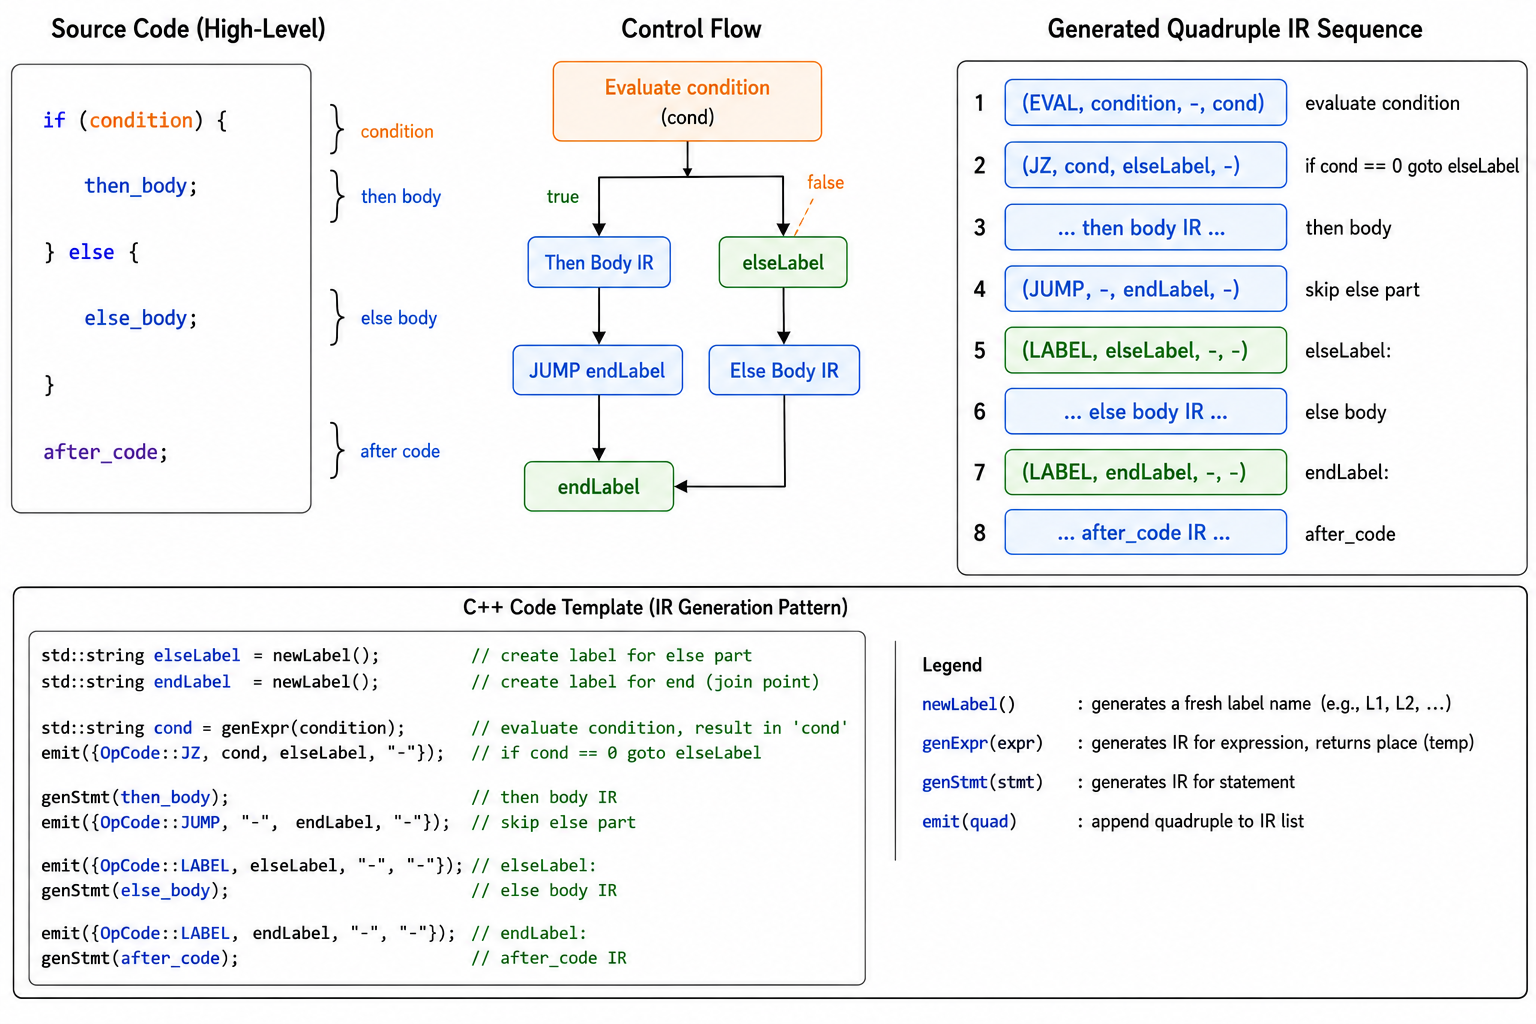
\includegraphics[width=0.65\linewidth]{screenshot009}
\caption{if语句的四元式翻译模式}
\label{fig:ir_if_pattern}
\end{figure}


\textbf{while语句翻译}：

\begin{lstlisting}[language=C++, caption={while语句IR生成}]
void genWhileStmt(const Node* node) {
    string startLabel = newLabel();  // 循环起始标签
    string endLabel = newLabel();    // 循环出口标签

    // Step 1: 循环起始标签
    emit(LABEL, startLabel);

    // Step 2: 生成条件IR → cond
    string cond = genExpr(conditionNode);

    // Step 3: cond为假 → 跳出循环
    emit(JZ, cond, endLabel);

    // Step 4: 设置break(→endLabel)和continue(→startLabel)
    string oldBreak = break_label;
    string oldContinue = continue_label;
    break_label = endLabel;
    continue_label = startLabel;

    // Step 5: 生成循环体的IR
    genBlock(bodyBlock);

    // Step 6: 循环体结束 → 跳回起始
    emit(JUMP, startLabel);

    // Step 7: 出口标签
    emit(LABEL, endLabel);

    // 恢复外层循环的break/continue标签
    break_label = oldBreak;
    continue_label = oldContinue;
}
\end{lstlisting}

\begin{figure}[H]
\centering
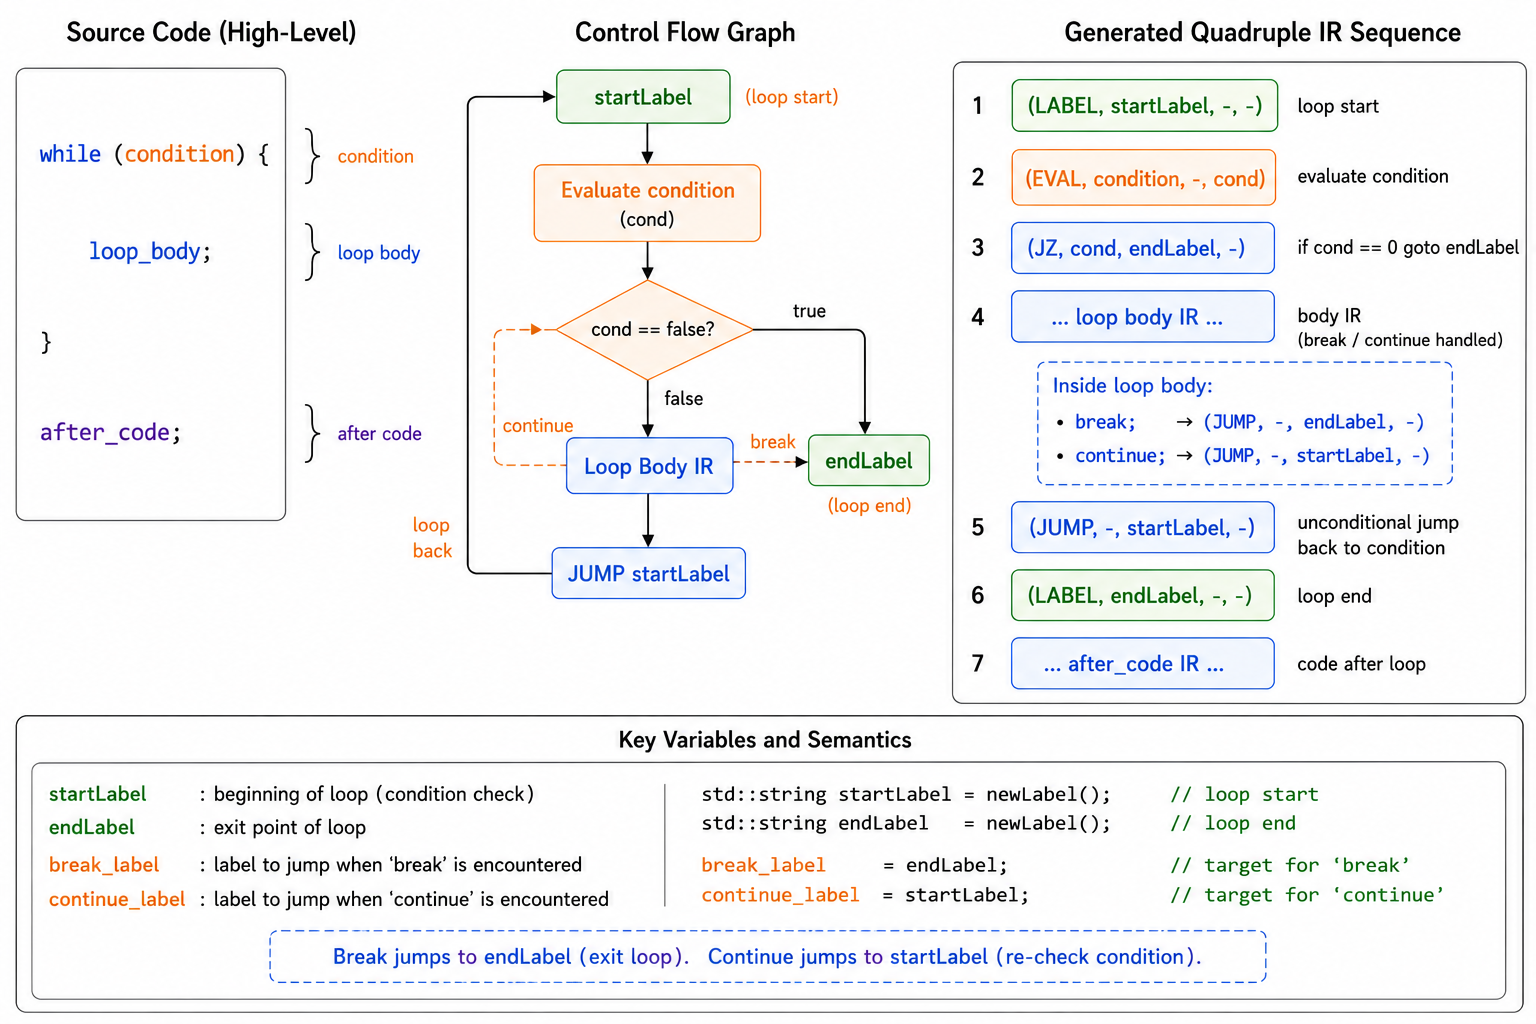
\includegraphics[width=0.65\linewidth]{screenshot010}
\caption{while语句的四元式翻译模式}
\label{fig:ir_while_pattern}
\end{figure}


\textbf{for语句翻译}：

for循环翻译为while循环的等价形式。以 \texttt{for mut i in start..end \{ body \}} 为例，翻译分为三个阶段：初始化（i=start）、条件判断（i<end）、递增（i=i+1）。

\begin{lstlisting}[language=IR, caption={for语句的四元式翻译模式}]
// === for mut i in start..end { body } ===
// 阶段1: 循环初始化（隐含的 i = start）
(ASSIGN, start, -, i)        // 因为for未显式写出，由IR生成器补全
(LABEL, for_start, -, -)      // 循环起始标签
(LT, i, end, cond)            // 循环条件: i < end ?
(JZ, cond, for_end)           // 不满足则跳出
// ... body IR ...
// continue跳转目标:
(LABEL, for_step, -, -)
(ADD, i, 1, i)                // i = i + 1（递增步长固定为1）
(JUMP, for_start, -, -)       // 跳回条件判断
(LABEL, for_end, -, -)        // 循环出口
\end{lstlisting}

注意for循环的continue标签指向step标签（而非start），这确保\texttt{continue}会先执行递增操作再检查条件，与Rust标准语义一致。

\textbf{嵌套if-else的翻译}：当if语句包含else-if链时，翻译模式递归展开。以\texttt{if a>0 \{...\} else if a<0 \{...\} else \{...\}} 为例：

\begin{lstlisting}[language=IR, caption={嵌套if-else的四元式翻译}]
// 计算外层条件 a > 0 → t0
(GT, a, 0, t0)
(JZ, t0, else_if_label)      // a<=0 → 跳到else if
// then分支 (a>0)
... then_body IR ...
(JUMP, end_label)             // 跳过所有else

(LABEL, else_if_label, -, -)
// 计算else-if条件 a < 0 → t1
(LT, a, 0, t1)
(JZ, t1, else_label)         // a>=0 → 跳到else
// else-if分支 (a<0)
... else_if_body IR ...
(JUMP, end_label)

(LABEL, else_label, -, -)
// else分支 (a==0)
... else_body IR ...

(LABEL, end_label, -, -)
\end{lstlisting}

这种翻译模式保证了三个分支的互斥执行：通过连续的JZ条件跳转链，每个分支的末尾以无条件JUMP跳过后续分支，形成清晰的if-else if-else控制流结构。

\textbf{loop语句翻译}：

loop是无限循环，只有显式的break能退出：

\begin{lstlisting}[language=IR, caption={loop语句的四元式翻译模式}]
(LABEL, loop_start, -, -)
// ... body IR ...
// break → (JUMP, loop_end)
// continue → (JUMP, loop_start)
(JUMP, loop_start, -, -)
(LABEL, loop_end, -, -)
\end{lstlisting}

\textbf{嵌套循环的break/continue处理}：

通过保存和恢复 \texttt{break\_label} 和 \texttt{continue\_label} 实现嵌套循环的支持：

\begin{lstlisting}[language=C++, caption={嵌套循环的break/continue标签管理}]
// 进入内层循环时保存外层标签
string oldBreak = break_label;
string oldContinue = continue_label;
break_label = endLabel;       // 内层break跳到内层出口
continue_label = startLabel;  // 内层continue跳到内层起始

// ... 生成内层循环体IR ...

// 离开内层循环时恢复外层标签
break_label = oldBreak;
continue_label = oldContinue;
\end{lstlisting}

\subsubsection{函数调用的IR生成}

函数调用涉及参数传递和返回值处理：

\begin{lstlisting}[language=C++, caption={函数调用IR生成}]
string genCallExpr(const Node* node) {
    string funcName = extractId(node);

    // Step 1: 为每个实参生成PARAM指令
    for (每个实参) {
        string argVal = genExpr(实参);
        emit(PARAM, argVal);
    }

    // Step 2: 生成CALL指令
    string result = newTemp();
    if (函数有返回值) {
        emit(CALL, funcName, 参数数量, result);
        return result;    // 返回临时变量持有函数结果
    } else {
        emit(CALL, funcName, 参数数量, "");
        return "";        // 无返回值
    }
}
\end{lstlisting}

例如，调用 \texttt{add(x, y)} 生成的四元式：
\begin{lstlisting}[language=IR]
(PARAM, x, -, -)
(PARAM, y, -, -)
(CALL, add, 2, t5)
\end{lstlisting}

\subsubsection{引用与解引用的IR生成}

\begin{lstlisting}[language=C++, caption={引用与解引用的IR生成}]
string genRefExpr(const Node* node) {
    string inner = genExpr(innerExpr);     // 被引用变量
    string result = newTemp();
    emit(REF, inner, "", result);          // result = &inner
    return result;
}

string genDerefExpr(const Node* node) {
    string inner = genExpr(innerExpr);     // 引用变量
    string result = newTemp();
    emit(DEREF, inner, "", result);        // result = *inner
    return result;
}
\end{lstlisting}

\subsection{完整的IR生成示例}

以 \texttt{fibonacci} 函数为例，展示完整程序的IR输出，并对每一段IR进行逐行解析：

\begin{lstlisting}[language=RustLike, caption={fibonacci函数源码（13行有效代码）}]
fn fibonacci(mut n:i32) -> i32 {
    if n<=1 { return n; }           // 基线条件
    let mut a:i32=0;                 // fib(0)
    let mut b:i32=1;                 // fib(1)
    let mut i:i32=2;                 // 循环计数器从2开始
    while i<=n {                      // 迭代计算
        let mut t:i32=a+b;           // t = fib(i)
        a=b;                         // fib(i-2) ← fib(i-1)
        b=t;                         // fib(i-1) ← fib(i)
        i=i+1;
    }
    return b;                        // 返回 fib(n)
}
\end{lstlisting}

该函数生成的IR共23条四元式：

\begin{lstlisting}[language=IR, caption={fibonacci函数的四元式IR（含逐行注释）}]
(0)  (FUNC_BEGIN, fibonacci, -, -)     // 函数入口标记
(1)  (ASSIGN, param_n, -, n)            // 接收参数: n = input
// === if n<=1 条件判断 ===
(2)  (LE, n, 1, t0)                     // t0 = (n <= 1)，比较运算结果存入临时变量
(3)  (JZ, t0, L0, -)                    // 若 t0 为假(n>1), 跳转到 L0 (跳过return)
// === then分支: return n ===
(4)  (RETURN, n, -, -)                  // n<=1时直接返回n (fib(0)=0, fib(1)=1)
(5)  (LABEL, L0, -, -)                  // 分支出口标签 (n>1时执行)
// === 初始化循环变量 ===
(6)  (ASSIGN, 0, -, a)                  // a = 0 (fib(0))
(7)  (ASSIGN, 1, -, b)                  // b = 1 (fib(1))
(8)  (ASSIGN, 2, -, i)                  // i = 2 (从第2项开始)
// === while i<=n 循环 ===
(9)  (LABEL, L1, -, -)                  // while 起始标签 (循环入口)
(10) (LE, i, n, t1)                     // t1 = (i <= n) 循环条件判断
(11) (JZ, t1, L2, -)                    // 条件为假, 跳出循环到 L2
// === 循环体: 斐波那契迭代 ===
(12) (ADD, a, b, t2)                    // t2 = a + b (当前斐波那契数)
(13) (ASSIGN, t2, -, t)                 // t = t2
(14) (ASSIGN, b, -, a)                  // a = b (右移: fib(k-2) ← fib(k-1))
(15) (ASSIGN, t, -, b)                  // b = t (右移: fib(k-1) ← fib(k))
(16) (ADD, i, 1, t3)                    // t3 = i + 1
(17) (ASSIGN, t3, -, i)                 // i = t3 (计数器递增)
(18) (JUMP, L1, -, -)                   // 无条件跳回循环起始 L1
// === 循环出口 ===
(19) (LABEL, L2, -, -)                  // while 出口标签
(20) (RETURN, b, -, -)                  // 返回 fib(n) = b
// === 函数收尾 ===
(21) (LABEL, func_fibonacci_end, -, -)  // 函数结束标签 (统一出口)
(22) (FUNC_END, fibonacci, -, -)        // 函数结束标记
\end{lstlisting}

\textbf{IR生成分析}：这23条IR展示了几个关键的翻译模式：
\begin{itemize}
    \item \textbf{参数传递}（行1）：函数参数通过特殊的\texttt{param\_n}形式映射到局部变量n
    \item \textbf{条件分支}（行2-5）：if语句的标准模式——计算条件→条件跳转→then体→标签出口
    \item \textbf{循环翻译}（行9-18）：while的标准模式——入口标签→条件判断→JZ跳出→循环体→无条件跳回→出口标签
    \item \textbf{表达式分解}（行12-17）：每个子表达式产生临时变量（t2, t3），赋值使用独立的ASSIGN指令
    \item \textbf{return收尾}（行21）：统一在函数末尾设置\texttt{func\_name\_end}标签，return语句在产生RETURN后也会跳转到此标签（函数内没有其他代码时省略JUMP）
\end{itemize}

从13行源码生成23条IR，平均每行源码约1.8条IR，这个比例反映了我们设计的IR粒度——既不冗余也不过粗。

\subsection{IR生成流程总览}

\begin{figure}[H]
\centering
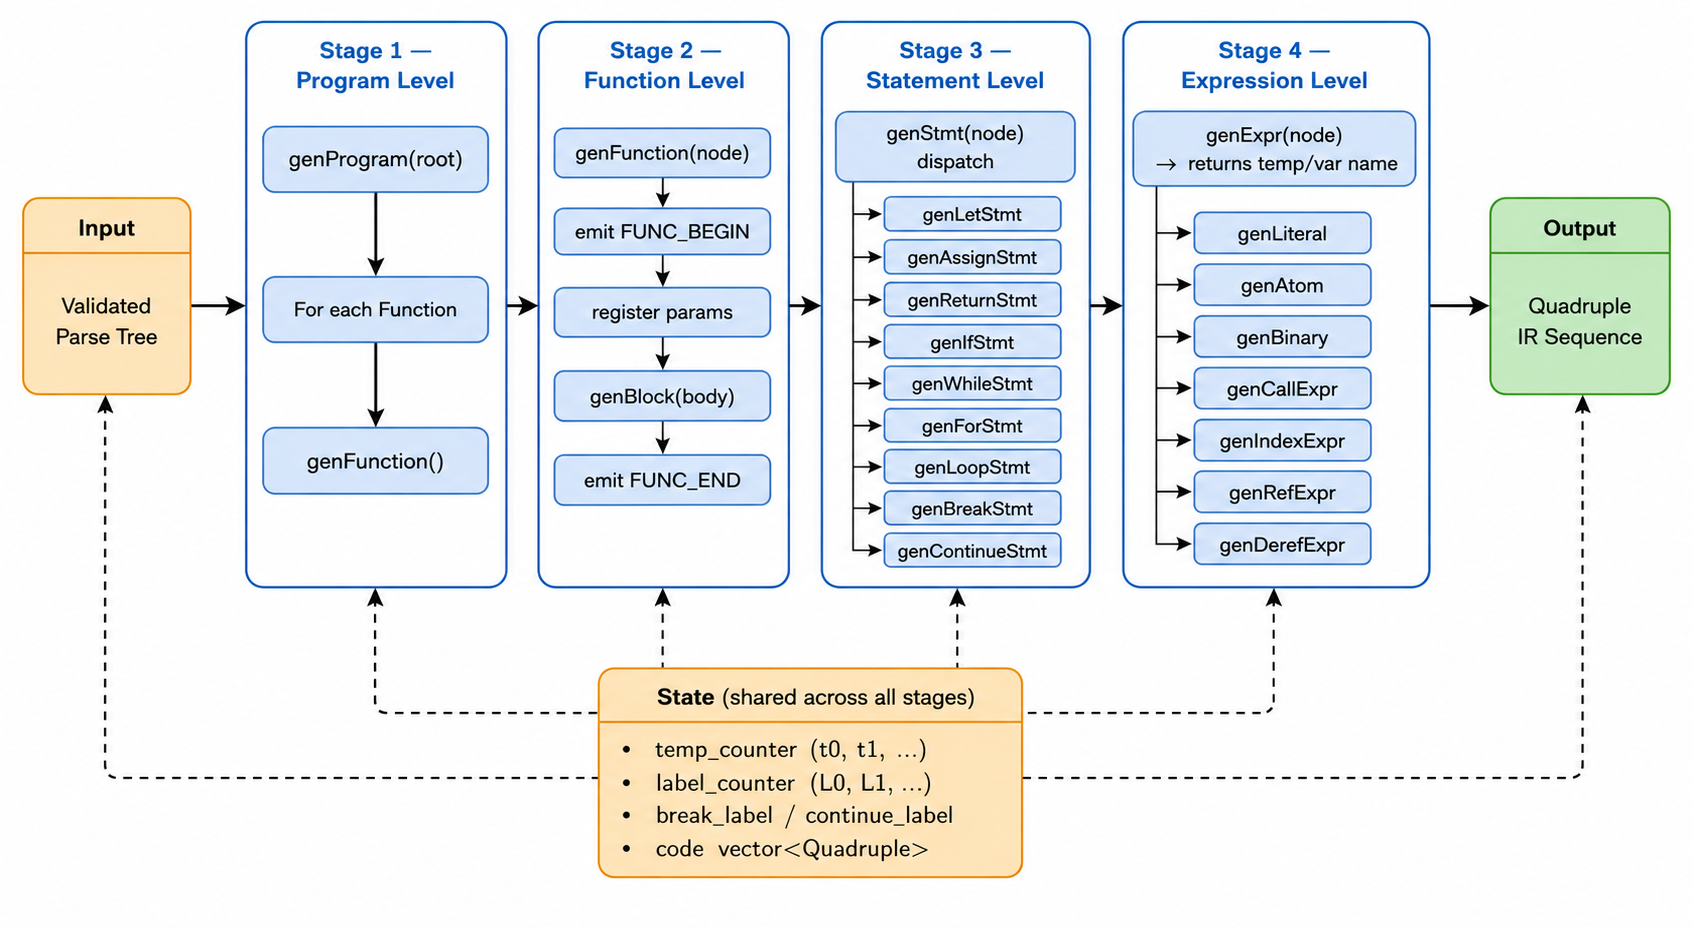
\includegraphics[width=\textwidth]{screenshot011}
\caption{中间代码生成整体流程图}
\label{fig:ir_flow}
\end{figure}


\newpage

% ============================================================
%  第四章 测试与结果分析
% ============================================================
\section{测试与结果分析}

本章通过完整的测试用例验证语义分析和中间代码生成的正确性。

\subsection{测试策略}

测试采用\textbf{集成测试}策略：完整的编译流水线（词法→语法→语义→IR）验证端到端正确性：

\begin{enumerate}
    \item \textbf{正向测试}（Pass tests）：编写语法和语义均正确的代码，验证分析通过并生成IR
    \item \textbf{负向测试}（Fail tests）：编写包含特定语义错误的代码，验证错误被正确检测
    \item \textbf{全规则覆盖}：确保每条作业要求中的语义规则都有对应的测试用例
\end{enumerate}

\subsection{测试用例设计}

\subsubsection{综合正确用例：test\_full.rs}

该文件包含30余个函数，覆盖全部必做规则（0.1--5.1）和选做规则（4.2--9.2），是语义分析的完整正确性验证：

\begin{lstlisting}[language=RustLike, caption={test\_full.rs 中的关键函数示例}]
// 1.5 函数输出
fn test_1_5() -> i32 {
    return 1;
}

// 2.3 变量声明赋值（含shadowing）
fn test_2_3() {
    let mut a:i32=1;
    let mut b=2;
    let mut a=3;           // shadowing
}

// 6.3 可变引用
fn test_6_3(mut a:i32) {
    let mut b:&mut i32=&mut a;
}

// 综合用例：fibonacci
fn fibonacci(mut n:i32) -> i32 {
    if n<=1 { return n; }
    let mut a:i32=0;
    let mut b:i32=1;
    let mut i:i32=2;
    while i<=n {
        let mut t:i32=a+b;
        a=b; b=t; i=i+1;
    }
    return b;
}
\end{lstlisting}

\textbf{测试结果}：test\_full.rs 通过语义分析，无错误报告，并成功生成97行四元式IR。

\subsubsection{语义错误检测用例：test\_errors.rs}

该文件包含17个函数，每个函数恰好触发一类语义错误：

\begin{lstlisting}[language=RustLike, caption={test\_errors.rs 语义错误测试}]
// 错误1,2: 返回类型不一致
fn err_1_5a() -> i32 { return ; }        // void→i32
fn err_1_5b() { return 1; }              // i32→void

// 错误3: 赋值给未声明变量
fn err_2_2a() { a=32; }

// 错误6: 不可变变量二次赋值
fn err_6_1() { let c:i32=1; c=2; }

// 错误13: 可变引用与不可变引用共存
fn err_6_3a() {
    let mut a:i32=1;
    let b=&a; let mut c=&mut a;
}

// 错误17: 数组初始化元素数量不一致
fn err_8_2a(mut a:i32) {
    let mut a:[i32;2];
    a=[1,2,3];
}
\end{lstlisting}

\textbf{测试结果}：test\_errors.rs 中的全部17个函数均被正确检测出语义错误，每个函数精确产生一类错误信息。以下是实际运行时parser输出的部分错误信息：

\begin{lstlisting}[caption={语义错误检测实际输出（节选）}, basicstyle=\ttfamily\footnotesize]
=== Semantic Errors ===
Error: return statement type (void) does not match function
       return type (i32) at line 2
Error: return statement type (i32) does not match function
       return type (void) at line 6
Error: variable 'a' not declared at line 10
Error: type mismatch in assignment: i32 vs bool at line 14
Error: variable 'a' not declared at line 18
Error: variable 'a' used before assignment at line 23
Error: cannot assign to immutable variable 'c' at line 29
Error: function 'err_3_5a_helper' expects 0 argument(s)
       but got 1 at line 34
Error: cannot use void expression as initializer at line 40
Error: argument 1 type mismatch in call to
       'err_3_5c_helper': expected i32 but got bool at line 46
Error: break statement must be inside a loop at line 50
Error: continue statement must be inside a loop at line 54
Error: cannot create mutable reference to 'a':
       other references already exist at line 60
Error: cannot create mutable reference to
       immutable variable 'a' at line 66
Error: cannot dereference non-reference type: i32 at line 71
Error: cannot assign through immutable reference at line 77
Error: type mismatch in assignment: [i32;2] vs [i32;3] at line 82
Error: type mismatch in assignment: (i32,i32) vs (i32,i32,i32)
       at line 87
\end{lstlisting}

每条错误信息都包含\textbf{错误描述}和\textbf{行号定位}，便于开发者快速定位问题。错误信息中的类型名称使用可读的字符串表示（如\texttt{[i32;2]}、\texttt{(i32,i32)}），而非内部枚举编号。

\subsection{批量测试脚本与结果}

\begin{lstlisting}[language=bash, caption={semantic\_tests.sh 测试脚本结构}]
#!/bin/bash
PARSER="./build/bin/parser"
PASS=0; FAIL=0; TOTAL=0

run_test() {
    # 运行parser，检查exit code
    # expect_pass="pass" 时期望exit code=0
    # expect_pass="fail" 时期望exit code≠0
}

# Rule 1.x: 程序结构 (7 tests)
# Rule 2.x: 变量声明与赋值 (4 tests)
# Rule 3.x: 表达式 (2 tests)
# Rule 3.5: 函数调用 (2 tests)
# Rule 4.x: 选择结构 (1 test)
# Rule 5.x: 循环 (3 tests)
# Rule 6.x: 引用 (2 tests)
# Rule 8.x: 数组 (1 test)
# Rule 9.x: 元组 (1 test)
# Total: 22 tests
\end{lstlisting}

\begin{table}[H]
\centering
\caption{测试结果汇总}
\begin{tabular}{|c|c|c|c|}
\hline
\textbf{测试规则范围} & \textbf{测试数量} & \textbf{通过} & \textbf{结果} \\
\hline
规则 1.x (程序结构) & 7 & 7 & \textcolor{green!60!black}{\checkmark} \\
\hline
规则 2.x (变量声明与赋值) & 4 & 4 & \textcolor{green!60!black}{\checkmark} \\
\hline
规则 3.x (表达式) & 2 & 2 & \textcolor{green!60!black}{\checkmark} \\
\hline
规则 3.5 (函数调用) & 2 & 2 & \textcolor{green!60!black}{\checkmark} \\
\hline
规则 4.x (选择结构) & 1 & 1 & \textcolor{green!60!black}{\checkmark} \\
\hline
规则 5.x (循环) & 3 & 3 & \textcolor{green!60!black}{\checkmark} \\
\hline
规则 6.x (引用) & 2 & 2 & \textcolor{green!60!black}{\checkmark} \\
\hline
规则 8.x (数组) & 1 & 1 & \textcolor{green!60!black}{\checkmark} \\
\hline
规则 9.x (元组) & 1 & 1 & \textcolor{green!60!black}{\checkmark} \\
\hline
\textbf{合计} & \textbf{22} & \textbf{22} & \textbf{100\%} \\
\hline
\end{tabular}
\end{table}

\subsection{运行效果}

\begin{figure}[H]
\centering
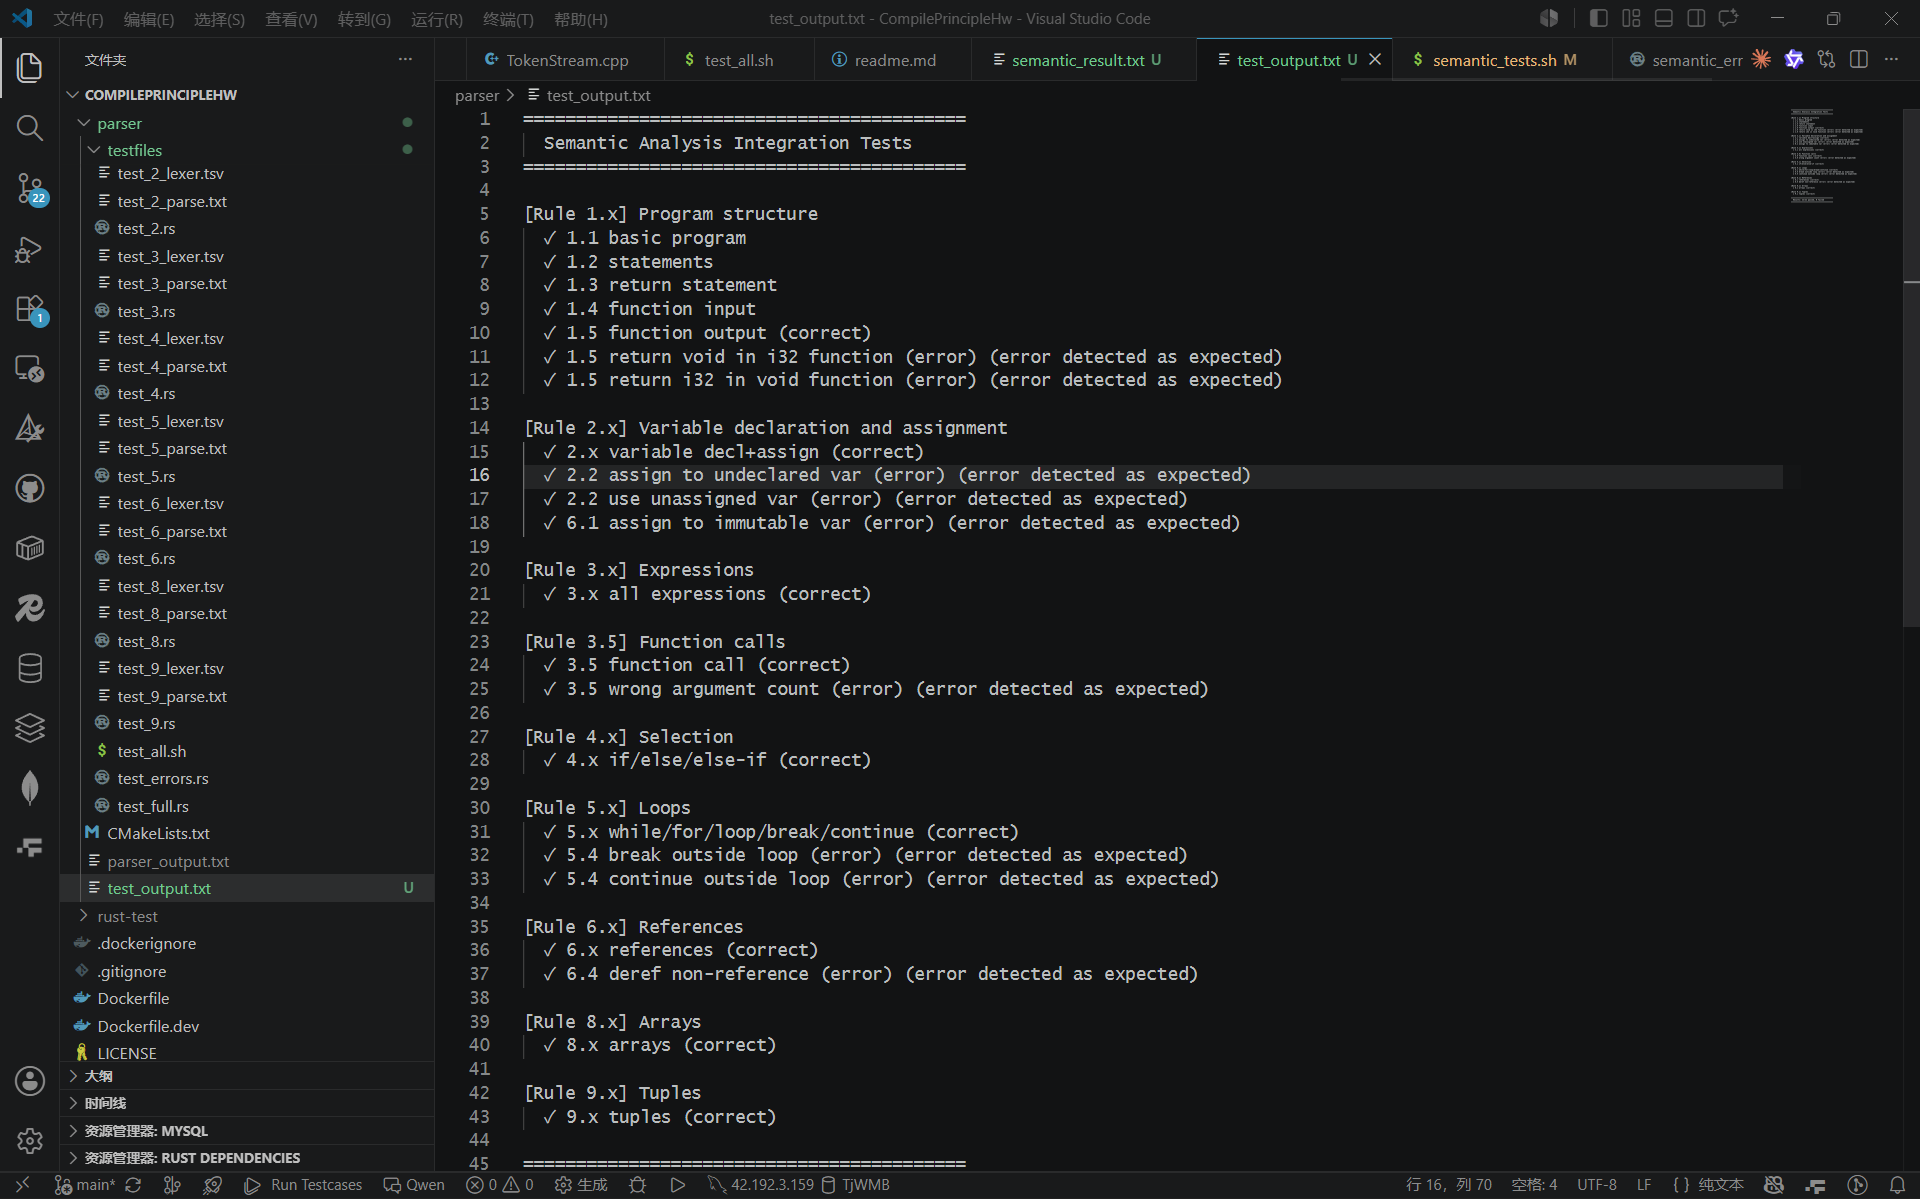
\includegraphics[width=\textwidth]{screenshot012}
\caption{命令行语义分析测试运行截图（22项测试全部通过）}
\label{fig:cli_test}
\end{figure}


\newpage

% ============================================================
%  第五章 思考与分析
% ============================================================
\section{思考与分析}

\subsection{语义分析中 Visitor 模式的设计考量}

\subsubsection{为什么选择 Visitor 模式}

在实现语义分析时，我们面临两种主要的设计选择：

\begin{enumerate}
    \item \textbf{在语法树节点中直接添加分析方法}：在Node类中添加virtual analyze方法
    \item \textbf{使用外部Visitor类}：将语义分析逻辑集中到独立的SemanticAnalyzer类中
\end{enumerate}

我们选择了方案2（Visitor模式），主要理由：
\begin{itemize}
    \item \textbf{关注点分离}：语法树节点仅负责存储结构，分析与生成逻辑独立
    \item \textbf{可扩展性}：可以方便地添加新的分析Pass（如后续的优化Pass）而不修改Node类
    \item \textbf{Info passing}：表达式Visitor可以返回值（类型信息），语句Visitor无需返回值，这种差异在Visitor模式中自然表达
\end{itemize}

\subsubsection{表达式类型传播的设计}

在实现中，所有\texttt{visitXxxExpr}方法返回\texttt{STypePtr}，沿语法树自底向上传播类型信息。这种设计的优势：
\begin{itemize}
    \item 表达式类型推导自然：字面量→基本类型，运算符→结果类型，标识符→查符号表
    \item 类型检查位置明确：在赋值、传参、返回等节点比较左右类型
    \item 代码可读性高：每个visit方法的返回值直接表达"这个子树求值后的类型"
\end{itemize}

\subsection{两遍扫描 vs 单遍扫描的权衡}

处理函数前向引用有两个常见策略：

\begin{enumerate}
    \item \textbf{两遍扫描}：先收集所有声明（函数签名、类型定义），再分析函数体
    \item \textbf{单遍扫描 + 待决列表}：遇到未定义的函数调用时，记录到待决列表，待函数定义后回填
\end{enumerate}

我们选择了方案1，原因如下：
\begin{itemize}
    \item \textbf{实现简单}：两遍扫描逻辑清晰，不需要处理复杂的待决回填
    \item \textbf{语义正确}：在我们的语言中，函数声明位于顶层，不存在嵌套函数，两遍扫描天然正确
    \item \textbf{与Rust行为一致}：Rust允许函数在任何位置定义，不做前向声明要求
\end{itemize}

方案1的代价是额外的语法树遍历（第一遍注册签名），但由于语法树已在内存中，第二遍遍历的开销可以接受。

\subsection{借用追踪的简化实现与局限}

本项目的借用追踪使用了\textbf{标志位方法}（has\_immutable\_ref / has\_mutable\_ref），在每个变量的符号表条目中记录当前存在的引用类型。这种实现能够检测作业要求的所有借用错误场景：

\begin{itemize}
    \item 可变引用与其他引用共存 → 检测到has\_immutable\_ref==true
    \item 从不可变变量创建可变引用 → 检测到is\_mutable==false
    \item 不可变引用修改数据 → 在赋值左侧检测ref类型
\end{itemize}

但与Rust编译器完整的\textbf{借用检查器}（Borrow Checker，基于NLL非词法生命周期）相比，我们的实现有以下局限：

\begin{enumerate}
    \item \textbf{未追踪引用的生命周期}：标志位一旦设置就不会清除，即使引用已经超出作用域
    \item \textbf{未处理函数间的借用}：函数参数和返回值的借用关系未做跨函数分析
    \item \textbf{简化了所有权模型}：我们的语言只支持i32类型（Copy语义），不涉及move语义和所有权转移
\end{enumerate}

这些简化是合理的——作业要求的语言子集不需要完整的Rust借用检查器，当前的实现完全覆盖了作业中的借用规则检测需求。

\subsection{四元式 vs 其他IR形式的对比}

我们选择四元式作为IR形式，与其他常见IR形式对比：

\begin{table}[H]
\centering
\caption{IR形式对比}
\begin{tabular}{|l|l|l|l|}
\hline
\textbf{IR形式} & \textbf{表示} & \textbf{优点} & \textbf{缺点} \\
\hline
四元式 & (op, a1, a2, r) & 实现简单，输出清晰 & 临时变量多，优化需额外处理 \\
\hline
三元式 & (op, a1, a2) & 无临时变量 & 移动代码时需更新引用 \\
\hline
间接三元式 & (op, a1, a2)+间接表 & 优化友好 & 实现复杂 \\
\hline
SSA形式 & 基于φ函数 & 优化最自然 & 实现复杂，对课程要求过重 \\
\hline
\end{tabular}
\end{table}

四元式是编译原理教材中最经典的形式，适合教学演示。每条指令的结果有独立的存储位置（临时变量），便于后续优化Pass（如公共子表达式消除、常量传播）对指令进行重排序和删除。

\subsection{控制流翻译中标签管理的设计}

控制流翻译的核心是\textbf{标签管理}。我们的设计中，break和continue的跳转目标通过两个变量（break\_label, continue\_label）存储，在进入嵌套循环时保存/恢复：

\begin{lstlisting}[language=C++, caption={嵌套循环的标签栈管理}]
// 伪代码：进入内层循环时
string oldBreak = break_label;     // 保存外层break目标
break_label = innerEndLabel;       // 内层break指向内层循环出口

genBlock(innerBody);

break_label = oldBreak;            // 恢复外层break目标
\end{lstlisting}

这种\textbf{单层保存}策略（而非完整的标签栈）之所以足够，是因为我们的程序设计使得每次进入循环体时就确定了break/continue目标，离开循环体时就恢复——本质上是一个隐式栈，通过函数调用栈来实现。这种设计简洁且在正确的递归生成IR代码时行为正确。

\subsection{语义错误的组织与报告策略}

语义分析器的错误处理采用\textbf{先收集、后报告}的策略：

\begin{enumerate}
    \item \textbf{收集阶段}：所有\texttt{error()}调用将错误信息追加到内部\texttt{vector<SemanticError>}，而非立即抛出异常。这使得语义分析可以继续运行，检测更多错误
    \item \textbf{报告阶段}：分析完成后，由\texttt{main.cpp}调用\texttt{analyzer.hasErrors()}判断是否存在任何错误。如有错误，调用\texttt{analyzer.printErrors()}统一输出
    \item \textbf{阻断策略}：一旦存在语义错误，IR生成阶段被跳过（main.cpp中\texttt{return 1}）。这是因为在存在语义错误的程序上生成IR可能导致后续阶段的行为未定义
\end{enumerate}

这种策略与工业编译器（如GCC的\texttt{-Werror}、Rust的rustc）一致：尽可能多地发现错误，一次性报告给用户，避免"修复一个错误又出现另一个"的低效循环。不过，当前实现的一个限制是：遇到错误后某些后续检查可能被跳过（如符号表条目缺失导致后续访问该符号的检查无法进行），这是\textbf{错误恢复}（Error Recovery）能力的不足，可作为改进方向。

\subsection{类型系统的设计哲学：结构化 vs 命名化}

我们在类型系统中做的一个关键设计选择是采用\textbf{结构化类型等价}（Structural Type Equivalence）而非\textbf{命名类型等价}（Nominal Type Equivalence）。具体体现在：

\begin{itemize}
    \item 两个\texttt{[i32; 3]}类型总是等价，无论它们声明在何处
    \item 两个\texttt{(i32, i32)} 元组类型总是等价
    \item 类型没有"名字"概念——比较的是类型的\textbf{内部结构}而非\textbf{外部名称}
\end{itemize}

这种选择是合理的，因为我们的语言没有\texttt{type}别名或用户自定义类型（如struct），所有类型都是内建的组合类型。如果未来扩展支持用户自定义类型，可能需要引入命名等价的概念来区分"结构相同但语义不同"的类型。

\subsection{IR操作码设计中的冗余与完备性}

回顾27种IR操作码的设计，可以发现一些有趣的设计模式：

\begin{itemize}
    \item \textbf{对称性}：算术运算（ADD/SUB/MUL/DIV）和比较运算（EQ/NE/LT/LE/GT/GE）各包含一组完备的操作。六个比较运算符构成了完整的偏序关系集合
    \item \textbf{最小完备性}：理论上JZ和JUMP就足以表达所有控制流（JNZ = JZ的取反、循环和分支可用JZ+JUMP实现），但我们仍然提供了JNZ以简化某些场景的IR生成（如逻辑与的短路求值）。BREAK和CONTINUE也可以归约为JUMP，但保留它们使IR更具可读性
    \item \textbf{数据操作层次}：INDEX\_LOAD/STORE、REF/DEREF构成了引用和复合类型操作的基础。ARRAY\_LIT的引入是为了统一处理数组字面量初始化——每个元素调用一次ARRAY\_LIT而非生成N条ASSIGN，这样既清晰又为后续的数组初始化优化留出了空间
\end{itemize}

IR设计的艺术在于在"太少"和"太多"之间找到平衡：太少则IR表达能力不足；太多则后续优化和代码生成需要处理过多case。我们的27种操作码是经过对语言特性的仔细分析后确定的——每个操作码都有清晰的语义和独立的存在价值。

\newpage

% ============================================================
%  第六章 总结与反思
% ============================================================
\section{总结与反思}

\subsection{项目成果总结}

本项目在前一阶段词法分析和语法分析的基础上，成功实现了语义分析器和中间代码生成器，完成了从源代码到中间代码的完整编译前端流水线。主要成果包括：

\begin{enumerate}
    \item \textbf{语义分析器}：基于Visitor模式实现了完整的类型检查和语义错误诊断，覆盖18类语义错误
    \item \textbf{类型系统}：设计了支持7种基础类型的类型层次结构，支持类型推导和类型一致性判断
    \item \textbf{符号表}：实现了栈式作用域管理，支持变量shadowing和借用追踪
    \item \textbf{中间代码生成器}：实现了四元式形式的IR生成，覆盖27种操作码
    \item \textbf{控制流翻译}：正确翻译if/else/while/for/loop/break/continue等控制流结构
    \item \textbf{完整测试}：22项集成测试全部通过，覆盖全部必做+选做规则
\end{enumerate}

\subsection{遇到的困难与解决方案}

\begin{enumerate}
    \item \textbf{函数前向引用问题}

    \textbf{问题}：如果函数A调用了后面定义的函数B，单遍扫描时B的签名尚未注册，导致"函数未声明"的误报。

    \textbf{解决方案}：采用两遍扫描策略。第一遍遍历所有函数头声明，注册签名到全局函数表；第二遍再分析函数体。这种方法简单有效，正确处理了前向引用。

    \item \textbf{类型系统的递归结构}

    \textbf{问题}：类型可以是嵌套的，如\texttt{[[i32;3];3]}（数组的数组）、\texttt{\&mut [i32;3]}（可变引用指向数组）。类型解析需要递归处理。

    \textbf{解决方案}：使用\texttt{shared\_ptr<SType>}实现类型的安全共享和递归引用。\texttt{parseTypeFromNode()}方法递归解析嵌套类型，inner指针指向内部类型。

    \item \textbf{借用追踪的标志位清除}

    \textbf{问题}：在最初的实现中，借用标志位设置后不会清除，导致后续对同一变量的合法操作被误报为错误。

    \textbf{解决方案}：调整了错误检测的触发条件，确保只在实际"创建引用时已有冲突引用存在"时才报错，而非在后续操作中报错。

    \item \textbf{四元式的arg2参数处理}

    \textbf{问题}：不同操作码的arg2含义不同——JUMP的arg1是目标标签，JZ的arg2是目标标签，CALL的arg2是参数数量。容易混淆。

    \textbf{解决方案}：建立明确的约定文档：JUMP→arg1为目标；JZ/JNZ→arg1为条件，arg2为目标；CALL→arg1为函数名，arg2为参数个数。在toString()中空值统一输出"-"。
\end{enumerate}

\subsection{知识收获与能力提升}

通过本次项目实践，我们获得了以下收获：

\begin{enumerate}
    \item \textbf{语义分析的完整理解}：从符号表设计到类型检查算法，深入理解了编译器"理解程序含义"的过程
    \item \textbf{Visitor模式的实际应用}：体会了设计模式在编译器构造中的价值——分离数据与操作
    \item \textbf{中间代码的设计思维}：理解了四元式作为"通用汇编"的设计哲学，以及控制流结构的标准翻译模式
    \item \textbf{测试驱动开发}：通过错误测试用例驱动语义分析的开发，每增加一个错误检测就增加对应的测试用例
    \item \textbf{工程迭代能力}：在已有代码基础上的扩展能力——理解既有架构，在不破坏已有功能的前提下添加新功能
\end{enumerate}

\subsection{流水线编排与模块协作}

整个编译流水线的编排在\texttt{main.cpp}中完成，形成了清晰的分阶段处理流程：

\begin{lstlisting}[language=C++, caption={main.cpp中的编译流水线编排}]
// 阶段1: 词法分析 → Token序列
TokenStream ts = lex(input);
ts.remove_comments();

// 阶段2: 语法分析 → 语法树
Parser parser(ts);
NodePtr tree = parser.parse();

// 阶段3: 语义分析 → 错误列表 OR 验证通过
SemanticAnalyzer analyzer;
analyzer.analyze(tree.get());
if (analyzer.hasErrors()) {
    analyzer.printErrors(cout);
    return 1;  // 语义错误，终止后续阶段
}

// 阶段4: 中间代码生成 → 四元式序列
IRGenerator irgen;
irgen.generate(tree.get());
irgen.writeIR(ir_output);
\end{lstlisting}

这种编排体现了编译器设计的经典原则：\textbf{每个阶段只做一件事，输入和输出明确}。阶段之间通过\texttt{NodePtr}（语法树）作为唯一的数据桥梁——语法树是词法分析和语法分析的输出，也是语义分析和IR生成的输入。这种设计使得各阶段可以独立开发、独立测试。

\subsection{改进方向与展望}

项目仍有改进空间：

\begin{enumerate}
    \item \textbf{IR优化}：当前生成的IR未经过优化，存在大量冗余的临时变量和无用赋值。可添加基本块划分、死代码消除、常量折叠等优化Pass。例如，\texttt{a = 0; b = a;} 当前生成两条IR，但可优化为\texttt{a = 0; b = 0;}（常量传播），或将连续的ASSIGN链合并
    \item \textbf{更丰富的类型系统}：可扩展支持bool、f64、字符串等基础类型。当前比较运算返回ST\_BOOL，但bool类型不能作为变量类型声明（声明bool需通过\texttt{let b = 1==1}的类型推导），添加原生bool类型将使语言更完整
    \item \textbf{更严谨的借用检查}：引入NLL（Non-Lexical Lifetime）风格的借用检查，替代当前的简单标志位方法。这需要追踪每个引用的"活跃区间"（liveness range），而非简单的bool标志
    \item \textbf{目标代码生成}：将四元式IR进一步翻译为x86汇编或LLVM IR，完成完整的编译后端。四元式→汇编的翻译是经典的后端任务，涉及寄存器分配、指令选择、调用约定等
    \item \textbf{错误恢复}：语义分析器在遇到第一个错误后可继续分析（而非立即停止），报告所有语义错误。这需要错误恢复机制——例如，当符号表查不到变量时，不立即终止当前函数分析，而是假设一个"错误类型"继续分析，避免级联错误
    \item \textbf{优化IR的标签生成}：当前每个if/while都会生成一对标签（L0/L1, L2/L3...），即使某些标签最终未被引用（如没有else的if语句，elseLabel不会被作为跳转目标）。可添加标签清理Pass，移除无用的LABEL指令
\end{enumerate}

\subsection{个人想法与体会}

\subsubsection{对语义分析在编译器中地位的认识}

实现语义分析的过程让我们深刻体会到：语法正确 ≠ 程序正确。一个程序即使完全符合文法规则，也可能存在大量错误——类型不匹配、变量未声明、违反借用规则等。语义分析是编译器"理解"程序的第一步，也是后续正确生成代码的基础。

在我们的实现中，有一个重要的设计原则：\textbf{语义分析不通过，不生成IR}。即main.cpp中先运行语义分析，只有 \texttt{!analyzer.hasErrors()} 时才进入IR生成阶段。这与工业编译器（如Rust的rustc）的行为一致——类型检查失败会阻止后续阶段。

\subsubsection{对四元式设计的反思}

四元式设计的一个关键权衡是\textbf{操作的粒度}。操作码越细粒度（如将 \texttt{a=b+c} 分解为明确的ADD+ASSIGN），IR越接近机器指令，后续优化和代码生成越容易；但IR的条数也会急剧增加。

我们选择了适中的粒度：二元运算保留在一条四元式中（(ADD, b, c, t0)），而赋值需要额外的ASSIGN（(ASSIGN, t0, -, a)）。这比"一条IR完成a=b+c"更清晰，比"分解为取b、取c、加、存a四条IR"更简洁。这是一个在表达能力与IR规模之间的合理折中。

\subsubsection{对渐进式文法设计的理解}

本项目的文法设计采用典型的\textbf{分层拓展}方式：从最简单的空函数开始，逐层添加语句、表达式、控制流、引用、数组、元组。在实现语义分析时，这种分层结构的优势更加明显——每增加一层语法规则，对应的语义检查也可以分层添加。

例如，实现完基础表达式（3.1--3.4）的语义分析后，添加函数调用（3.5）只需要：
\begin{enumerate}
    \item 在visitExpr中添加CallExpr分支
    \item 实现visitCallExpr：查函数表→检查实参数量→逐个检查实参类型→返回函数的返回类型
    \item 添加对应的语义错误测试用例
\end{enumerate}

这种增量式的开发方式降低了复杂度，使得为一个已有语法正确性验证的系统添加语义分析成为可控的过程。

\newpage

% ============================================================
%  参考文献
% ============================================================
\section{参考文献}

\begin{enumerate}
    \item Alfred V. Aho, Monica S. Lam, Ravi Sethi, Jeffrey D. Ullman. 编译原理（第2版）. 机械工业出版社, 2009.
    \item Andrew W. Appel. Modern Compiler Implementation in C. Cambridge University Press, 1998.
    \item Rust程序设计语言（中文版）. \url{https://rustwiki.org/zh-CN/book/}
    \item Rust Reference — 借用检查. \url{https://doc.rust-lang.org/reference/}
    \item 北京大学编译实践课程在线文档. \url{https://pku-minic.github.io/online-doc/}
    \item 自己动手写编译器. \url{https://pandolia.net/tinyc/index.html}
    \item LLVM Language Reference Manual. \url{https://llvm.org/docs/LangRef.html}
    \item CLIUtils/CLI11: Command line parser for C++11. \url{https://github.com/CLIUtils/CLI11}
    \item antlr/grammars-v4: Rust grammar for ANTLR v4. \url{https://github.com/antlr/grammars-v4/tree/master/rust}
    \item ocornut/imgui: Dear ImGui. \url{https://github.com/ocornut/imgui}
\end{enumerate}

\newpage

% ============================================================
%  附录A：完整IR操作码定义
% ============================================================
\section*{附录A\quad 完整IR操作码定义表}
\addcontentsline{toc}{section}{附录A\quad 完整IR操作码定义表}

\begin{longtable}{|l|l|l|l|}
\caption{四元式操作码完整定义} \\
\hline
\textbf{操作码} & \textbf{arg1} & \textbf{arg2} & \textbf{语义} \\
\hline
\endfirsthead
\hline
\textbf{操作码} & \textbf{arg1} & \textbf{arg2} & \textbf{语义} \\
\hline
\endhead
\hline
\endfoot
\hline
\endlastfoot

FUNC\_BEGIN & 函数名 & - & 函数开始标记 \\
FUNC\_END & 函数名 & - & 函数结束标记 \\
\hline
LABEL & 标签名 & - & 定义跳转标签 \\
JUMP & 目标标签 & - & 无条件跳转 \\
JZ & 条件变量 & 目标标签 & 若条件为假则跳转 \\
JNZ & 条件变量 & 目标标签 & 若条件为真则跳转 \\
\hline
ASSIGN & 源值 & - & 赋值: result = arg1 \\
ADD & 左操作数 & 右操作数 & 加法: result = arg1 + arg2 \\
SUB & 左操作数 & 右操作数 & 减法: result = arg1 - arg2 \\
MUL & 左操作数 & 右操作数 & 乘法: result = arg1 * arg2 \\
DIV & 左操作数 & 右操作数 & 除法: result = arg1 / arg2 \\
NEG & 操作数 & - & 取负: result = -arg1 \\
\hline
EQ & 左操作数 & 右操作数 & 相等: result = (arg1 == arg2) \\
NE & 左操作数 & 右操作数 & 不等: result = (arg1 != arg2) \\
LT & 左操作数 & 右操作数 & 小于: result = (arg1 < arg2) \\
LE & 左操作数 & 右操作数 & 小于等于: result = (arg1 <= arg2) \\
GT & 左操作数 & 右操作数 & 大于: result = (arg1 > arg2) \\
GE & 左操作数 & 右操作数 & 大于等于: result = (arg1 >= arg2) \\
\hline
PARAM & 实参值 & - & 传递实参 \\
CALL & 函数名 & 参数个数 & 函数调用 \\
RETURN & 返回值 & - & 函数返回 \\
\hline
INDEX\_LOAD & 数组名 & 索引 & 读取数组元素: result = arg1[arg2] \\
INDEX\_STORE & 值 & 索引 & 写入数组元素: arg1[arg2] = arg3 \\
REF & 变量名 & - & 取引用: result = \&arg1 \\
DEREF & 引用名 & - & 解引用: result = *arg1 \\
ARRAY\_LIT & 元素值 & 位置 & 数组字面量元素填充 \\
TUPLE\_GET & 元组名 & 位置 & 元组元素访问 \\
\hline
BREAK & - & - & 跳出循环 \\
CONTINUE & - & - & 继续下一次循环 \\
NOP & - & - & 空操作 \\
\hline
\end{longtable}

\newpage

% ============================================================
%  附录B：完整测试用例索引
% ============================================================
\section*{附录B\quad 完整测试用例索引}
\addcontentsline{toc}{section}{附录B\quad 完整测试用例索引}

\begin{longtable}{|l|l|l|l|}
\caption{测试用例与覆盖规则对应表} \\
\hline
\textbf{测试文件} & \textbf{测试类型} & \textbf{覆盖规则} & \textbf{预期结果} \\
\hline
\endfirsthead
\hline
\textbf{测试文件} & \textbf{测试类型} & \textbf{覆盖规则} & \textbf{预期结果} \\
\hline
\endhead
\hline
\endfoot
\hline
\endlastfoot

test\_1\_1.rs & 语法+语义 & 1.1 & 通过 \\
test\_1\_2.rs & 语法+语义 & 1.2 & 通过 \\
test\_1\_3.rs & 语法+语义 & 1.3 & 通过 \\
test\_1\_4.rs & 语法+语义 & 1.4 & 通过 \\
test\_1\_5.rs & 语法+语义 & 1.5 & 通过 \\
test\_2.rs & 语法+语义 & 2.0--2.3 & 通过 \\
test\_3.rs & 语法+语义 & 3.1--3.5 & 通过 \\
test\_4.rs & 语法+语义 & 4.1--4.3 & 通过 \\
test\_5.rs & 语法+语义 & 5.0--5.4 & 通过 \\
test\_6.rs & 语法+语义 & 6.1--6.4 & 通过 \\
test\_8.rs & 语法+语义 & 8.1--8.3 & 通过 \\
test\_9.rs & 语法+语义 & 9.1--9.3 & 通过 \\
\hline
test\_full.rs & 语义分析综合 & 全规则 & 通过（无错误） \\
test\_errors.rs & 语义错误检测 & 18类错误 & 检测到全部错误 \\
\hline
\end{longtable}

\textbf{运行命令示例}

\begin{lstlisting}[language=bash, caption={完整流水线运行命令}]
# 语义分析 + IR生成
./parser --input test_full.rs \
    --semantic-output semantic.txt \
    --ir-output ir.txt

# 仅语法分析（向后兼容）
./parser --input input.rs \
    --lexer-output lex.tsv \
    --parser-output tree.txt

# 静默模式
./parser --input input.rs -q \
    --semantic-output semantic.txt \
    --ir-output ir.txt
\end{lstlisting}

\newpage


\end{document}
